%TODO: Chapter needs to be improved a lot
\documentclass[11pt,compress,t,notes=noshow, aspectratio=169, xcolor=table]{beamer}

\usepackage{../../style/lmu-lecture}
% Defines macros and environments
\usepackage[]{graphicx}
\usepackage[]{color}
% maxwidth is the original width if it is less than linewidth
% otherwise use linewidth (to make sure the graphics do not exceed the margin)
\makeatletter
\def\maxwidth{ %
\ifdim\Gin@nat@width>\linewidth
\linewidth
\else
\Gin@nat@width
\fi
}
\makeatother
%\usepackage[fontsize=10.5pt]{scrextend}
\definecolor{ggred}{rgb}{0.973, 0.463, 0.427}
\definecolor{ggblue}{rgb}{0, 0.749, 0.769}
\definecolor{fgcolor}{rgb}{0.345, 0.345, 0.345}
\newcommand{\hlnum}[1]{\textcolor[rgb]{0.686,0.059,0.569}{#1}}%
\newcommand{\hlstr}[1]{\textcolor[rgb]{0.192,0.494,0.8}{#1}}%
\newcommand{\hlcom}[1]{\textcolor[rgb]{0.678,0.584,0.686}{\textit{#1}}}%
\newcommand{\hlopt}[1]{\textcolor[rgb]{0,0,0}{#1}}%
\newcommand{\hlstd}[1]{\textcolor[rgb]{0.345,0.345,0.345}{#1}}%
\newcommand{\hlkwa}[1]{\textcolor[rgb]{0.161,0.373,0.58}{\textbf{#1}}}%
\newcommand{\hlkwb}[1]{\textcolor[rgb]{0.69,0.353,0.396}{#1}}%
\newcommand{\hlkwc}[1]{\textcolor[rgb]{0.333,0.667,0.333}{#1}}%
\newcommand{\hlkwd}[1]{\textcolor[rgb]{0.737,0.353,0.396}{\textbf{#1}}}%
\newcommand{\predvar}{Var\left[\hat{f}(\xv)\right]}
\let\hlipl\hlkwb

\usepackage{pdfpages}
\usepackage{framed}
\makeatletter
\newenvironment{kframe}{%
\def\at@end@of@kframe{}%
\ifinner\ifhmode%
\def\at@end@of@kframe{\end{minipage}}%
\begin{minipage}{\columnwidth}%
\fi\fi%
\def\FrameCommand##1{\hskip\@totalleftmargin \hskip-\fboxsep
\colorbox{shadecolor}{##1}\hskip-\fboxsep
% There is no \\@totalrightmargin, so:
\hskip-\linewidth \hskip-\@totalleftmargin \hskip\columnwidth}%
\MakeFramed {\advance\hsize-\width
\@totalleftmargin\z@ \linewidth\hsize
\@setminipage}}%
{\par\unskip\endMakeFramed%
\at@end@of@kframe}
\makeatother

\definecolor{shadecolor}{rgb}{.97, .97, .97}
\definecolor{messagecolor}{rgb}{0, 0, 0}
\definecolor{warningcolor}{rgb}{1, 0, 1}
\definecolor{errorcolor}{rgb}{1, 0, 0}
\newenvironment{knitrout}{}{} % an empty environment to be redefined in TeX

\usepackage{alltt}
\newcommand{\SweaveOpts}[1]{}  % do not interfere with LaTeX
\newcommand{\SweaveInput}[1]{} % because they are not real TeX commands
\newcommand{\Sexpr}[1]{}       % will only be parsed by R

\usepackage[english]{babel}
\usepackage[utf8]{inputenc}

\usepackage[export]{adjustbox}
\usepackage{dsfont}
\usepackage{verbatim}
\usepackage{amsmath}
\usepackage{amsfonts}
\usepackage{bm}
\usepackage{csquotes}
\usepackage{multirow}
\usepackage{longtable}
\usepackage{booktabs}
\usepackage{enumerate}
\usepackage[absolute,overlay]{textpos}
\usepackage{psfrag}
\usepackage{algorithm}
\usepackage{algpseudocode}
\usepackage{eqnarray}
\usepackage{arydshln}
\usepackage{tabularx}
\usepackage{placeins}
\usepackage{tikz}
\usepackage{setspace}
\usepackage{colortbl}
\usepackage{mathtools}
\usepackage{wrapfig}
\usepackage{bm}
\usepackage[backend=biber]{biblatex}

\usetikzlibrary{tikzmark, shapes,arrows,automata,positioning,calc,chains,trees,  shadows, decorations.pathreplacing}
\tikzset{
%Define standard arrow tip
>=stealth',
%Define style for boxes
punkt/.style={
rectangle,
rounded corners,
draw=black, very thick,
text width=6.5em,
minimum height=2em,
text centered},
% Define arrow style
pil/.style={
->,
thick,
shorten <=2pt,
shorten >=2pt,}
}

\usepackage{subfig}

\usepackage{bbm}
%\newcommand\hmmax{0}
%\newcommand\bmmax{0}
% basic latex stuff
\newcommand{\pkg}[1]{{\fontseries{b}\selectfont #1}} %fontstyle for R packages
\newcommand{\lz}{\vspace{0.5cm}} %vertical space
\newcommand{\dlz}{\vspace{1cm}} %double vertical space
\newcommand{\oneliner}[1] % Oneliner for important statements
{\begin{block}{}\begin{center}\begin{Large}#1\end{Large}\end{center}\end{block}}

% Latexmath Notation
% math spaces
\ifdefined\N                                                                
\renewcommand{\N}{\mathds{N}} % N, naturals
\else \newcommand{\N}{\mathds{N}} \fi 
\newcommand{\Z}{\mathds{Z}} % Z, integers
\newcommand{\Q}{\mathds{Q}} % Q, rationals
\newcommand{\R}{\mathds{R}} % R, reals
\ifdefined\C 
  \renewcommand{\C}{\mathds{C}} % C, complex
\else \newcommand{\C}{\mathds{C}} \fi
\newcommand{\continuous}{\mathcal{C}} % C, space of continuous functions
\newcommand{\M}{\mathcal{M}} % machine numbers
\newcommand{\epsm}{\epsilon_m} % maximum error

% counting / finite sets
\newcommand{\setzo}{\{0, 1\}} % set 0, 1
\newcommand{\setmp}{\{-1, +1\}} % set -1, 1
\newcommand{\unitint}{[0, 1]} % unit interval

% basic math stuff
\newcommand{\xt}{\tilde x} % x tilde
\newcommand{\argmax}{\operatorname{arg\,max}} % argmax
\newcommand{\argmin}{\operatorname{arg\,min}} % argmin
\newcommand{\argminlim}{\mathop{\mathrm{arg\,min}}\limits} % argmax with limits
\newcommand{\argmaxlim}{\mathop{\mathrm{arg\,max}}\limits} % argmin with limits  
\newcommand{\sign}{\operatorname{sign}} % sign, signum
\newcommand{\I}{\mathbb{I}} % I, indicator
\newcommand{\order}{\mathcal{O}} % O, order
\newcommand{\pd}[2]{\frac{\partial{#1}}{\partial #2}} % partial derivative
\newcommand{\floorlr}[1]{\left\lfloor #1 \right\rfloor} % floor
\newcommand{\ceillr}[1]{\left\lceil #1 \right\rceil} % ceiling

% sums and products
\newcommand{\sumin}{\sum\limits_{i=1}^n} % summation from i=1 to n
\newcommand{\sumim}{\sum\limits_{i=1}^m} % summation from i=1 to m
\newcommand{\sumjn}{\sum\limits_{j=1}^n} % summation from j=1 to p
\newcommand{\sumjp}{\sum\limits_{j=1}^p} % summation from j=1 to p
\newcommand{\sumik}{\sum\limits_{i=1}^k} % summation from i=1 to k
\newcommand{\sumkg}{\sum\limits_{k=1}^g} % summation from k=1 to g
\newcommand{\sumjg}{\sum\limits_{j=1}^g} % summation from j=1 to g
\newcommand{\meanin}{\frac{1}{n} \sum\limits_{i=1}^n} % mean from i=1 to n
\newcommand{\meanim}{\frac{1}{m} \sum\limits_{i=1}^m} % mean from i=1 to n
\newcommand{\meankg}{\frac{1}{g} \sum\limits_{k=1}^g} % mean from k=1 to g
\newcommand{\prodin}{\prod\limits_{i=1}^n} % product from i=1 to n
\newcommand{\prodkg}{\prod\limits_{k=1}^g} % product from k=1 to g
\newcommand{\prodjp}{\prod\limits_{j=1}^p} % product from j=1 to p

% linear algebra
\newcommand{\one}{\boldsymbol{1}} % 1, unitvector
\newcommand{\zero}{\mathbf{0}} % 0-vector
\newcommand{\id}{\boldsymbol{I}} % I, identity
\newcommand{\diag}{\operatorname{diag}} % diag, diagonal
\newcommand{\trace}{\operatorname{tr}} % tr, trace
\newcommand{\spn}{\operatorname{span}} % span
\newcommand{\scp}[2]{\left\langle #1, #2 \right\rangle} % <.,.>, scalarproduct
\newcommand{\mat}[1]{\begin{pmatrix} #1 \end{pmatrix}} % short pmatrix command
\newcommand{\Amat}{\mathbf{A}} % matrix A
\newcommand{\Deltab}{\mathbf{\Delta}} % error term for vectors

% basic probability + stats
\renewcommand{\P}{\mathds{P}} % P, probability
\newcommand{\E}{\mathds{E}} % E, expectation
\newcommand{\var}{\mathsf{Var}} % Var, variance
\newcommand{\cov}{\mathsf{Cov}} % Cov, covariance
\newcommand{\corr}{\mathsf{Corr}} % Corr, correlation
\newcommand{\normal}{\mathcal{N}} % N of the normal distribution
\newcommand{\iid}{\overset{i.i.d}{\sim}} % dist with i.i.d superscript
\newcommand{\distas}[1]{\overset{#1}{\sim}} % ... is distributed as ...

% machine learning
\newcommand{\Xspace}{\mathcal{X}} % X, input space
\newcommand{\Yspace}{\mathcal{Y}} % Y, output space
\newcommand{\nset}{\{1, \ldots, n\}} % set from 1 to n
\newcommand{\pset}{\{1, \ldots, p\}} % set from 1 to p
\newcommand{\gset}{\{1, \ldots, g\}} % set from 1 to g
\newcommand{\Pxy}{\mathbb{P}_{xy}} % P_xy
\newcommand{\Exy}{\mathbb{E}_{xy}} % E_xy: Expectation over random variables xy
\newcommand{\xv}{\mathbf{x}} % vector x (bold)
\newcommand{\xtil}{\tilde{\mathbf{x}}} % vector x-tilde (bold)
\newcommand{\yv}{\mathbf{y}} % vector y (bold)
\newcommand{\xy}{(\xv, y)} % observation (x, y)
\newcommand{\xvec}{\left(x_1, \ldots, x_p\right)^\top} % (x1, ..., xp) 
\newcommand{\Xmat}{\mathbf{X}} % Design matrix
\newcommand{\allDatasets}{\mathds{D}} % The set of all datasets
\newcommand{\allDatasetsn}{\mathds{D}_n}  % The set of all datasets of size n 
\newcommand{\D}{\mathcal{D}} % D, data
\newcommand{\Dn}{\D_n} % D_n, data of size n
\newcommand{\Dtrain}{\mathcal{D}_{\text{train}}} % D_train, training set
\newcommand{\Dtest}{\mathcal{D}_{\text{test}}} % D_test, test set
\newcommand{\xyi}[1][i]{\left(\xv^{(#1)}, y^{(#1)}\right)} % (x^i, y^i), i-th observation
\newcommand{\Dset}{\left( \xyi[1], \ldots, \xyi[n]\right)} % {(x1,y1)), ..., (xn,yn)}, data
\newcommand{\defAllDatasetsn}{(\Xspace \times \Yspace)^n} % Def. of the set of all datasets of size n 
\newcommand{\defAllDatasets}{\bigcup_{n \in \N}(\Xspace \times \Yspace)^n} % Def. of the set of all datasets 
\newcommand{\xdat}{\left\{ \xv^{(1)}, \ldots, \xv^{(n)}\right\}} % {x1, ..., xn}, input data
\newcommand{\ydat}{\left\{ \yv^{(1)}, \ldots, \yv^{(n)}\right\}} % {y1, ..., yn}, input data
\newcommand{\yvec}{\left(y^{(1)}, \hdots, y^{(n)}\right)^\top} % (y1, ..., yn), vector of outcomes
\renewcommand{\xi}[1][i]{\xv^{(#1)}} % x^i, i-th observed value of x
\newcommand{\yi}[1][i]{y^{(#1)}} % y^i, i-th observed value of y 
\newcommand{\xivec}{\left(x^{(i)}_1, \ldots, x^{(i)}_p\right)^\top} % (x1^i, ..., xp^i), i-th observation vector
\newcommand{\xj}{\xv_j} % x_j, j-th feature
\newcommand{\xjvec}{\left(x^{(1)}_j, \ldots, x^{(n)}_j\right)^\top} % (x^1_j, ..., x^n_j), j-th feature vector
\newcommand{\phiv}{\mathbf{\phi}} % Basis transformation function phi
\newcommand{\phixi}{\mathbf{\phi}^{(i)}} % Basis transformation of xi: phi^i := phi(xi)

%%%%%% ml - models general
\newcommand{\lamv}{\bm{\lambda}} % lambda vector, hyperconfiguration vector
\newcommand{\Lam}{\bm{\Lambda}}	 % Lambda, space of all hpos
% Inducer / Inducing algorithm
\newcommand{\preimageInducer}{\left(\defAllDatasets\right)\times\Lam} % Set of all datasets times the hyperparameter space
\newcommand{\preimageInducerShort}{\allDatasets\times\Lam} % Set of all datasets times the hyperparameter space
% Inducer / Inducing algorithm
\newcommand{\ind}{\mathcal{I}} % Inducer, inducing algorithm, learning algorithm 

% continuous prediction function f
\newcommand{\ftrue}{f_{\text{true}}}  % True underlying function (if a statistical model is assumed)
\newcommand{\ftruex}{\ftrue(\xv)} % True underlying function (if a statistical model is assumed)
\newcommand{\fx}{f(\xv)} % f(x), continuous prediction function
\newcommand{\fdomains}{f: \Xspace \rightarrow \R^g} % f with domain and co-domain
\newcommand{\Hspace}{\mathcal{H}} % hypothesis space where f is from
\newcommand{\fbayes}{f^{\ast}} % Bayes-optimal model
\newcommand{\fxbayes}{f^{\ast}(\xv)} % Bayes-optimal model
\newcommand{\fkx}[1][k]{f_{#1}(\xv)} % f_j(x), discriminant component function
\newcommand{\fh}{\hat{f}} % f hat, estimated prediction function
\newcommand{\fxh}{\fh(\xv)} % fhat(x)
\newcommand{\fxt}{f(\xv ~|~ \thetab)} % f(x | theta)
\newcommand{\fxi}{f\left(\xv^{(i)}\right)} % f(x^(i))
\newcommand{\fxih}{\hat{f}\left(\xv^{(i)}\right)} % f(x^(i))
\newcommand{\fxit}{f\left(\xv^{(i)} ~|~ \thetab\right)} % f(x^(i) | theta)
\newcommand{\fhD}{\fh_{\D}} % fhat_D, estimate of f based on D
\newcommand{\fhDtrain}{\fh_{\Dtrain}} % fhat_Dtrain, estimate of f based on D
\newcommand{\fhDnlam}{\fh_{\Dn, \lamv}} %model learned on Dn with hp lambda
\newcommand{\fhDlam}{\fh_{\D, \lamv}} %model learned on D with hp lambda
\newcommand{\fhDnlams}{\fh_{\Dn, \lamv^\ast}} %model learned on Dn with optimal hp lambda 
\newcommand{\fhDlams}{\fh_{\D, \lamv^\ast}} %model learned on D with optimal hp lambda 

% discrete prediction function h
\newcommand{\hx}{h(\xv)} % h(x), discrete prediction function
\newcommand{\hh}{\hat{h}} % h hat
\newcommand{\hxh}{\hat{h}(\xv)} % hhat(x)
\newcommand{\hxt}{h(\xv | \thetab)} % h(x | theta)
\newcommand{\hxi}{h\left(\xi\right)} % h(x^(i))
\newcommand{\hxit}{h\left(\xi ~|~ \thetab\right)} % h(x^(i) | theta)
\newcommand{\hbayes}{h^{\ast}} % Bayes-optimal classification model
\newcommand{\hxbayes}{h^{\ast}(\xv)} % Bayes-optimal classification model

% yhat
\newcommand{\yh}{\hat{y}} % yhat for prediction of target
\newcommand{\yih}{\hat{y}^{(i)}} % yhat^(i) for prediction of ith targiet
\newcommand{\resi}{\yi- \yih}

% theta
\newcommand{\thetah}{\hat{\theta}} % theta hat
\newcommand{\thetab}{\bm{\theta}} % theta vector
\newcommand{\thetabh}{\bm{\hat\theta}} % theta vector hat
\newcommand{\thetat}[1][t]{\thetab^{[#1]}} % theta^[t] in optimization
\newcommand{\thetatn}[1][t]{\thetab^{[#1 +1]}} % theta^[t+1] in optimization
\newcommand{\thetahDnlam}{\thetabh_{\Dn, \lamv}} %theta learned on Dn with hp lambda
\newcommand{\thetahDlam}{\thetabh_{\D, \lamv}} %theta learned on D with hp lambda
\newcommand{\mint}{\min_{\thetab \in \Theta}} % min problem theta
\newcommand{\argmint}{\argmin_{\thetab \in \Theta}} % argmin theta

% densities + probabilities
% pdf of x 
\newcommand{\pdf}{p} % p
\newcommand{\pdfx}{p(\xv)} % p(x)
\newcommand{\pixt}{\pi(\xv~|~ \thetab)} % pi(x|theta), pdf of x given theta
\newcommand{\pixit}[1][i]{\pi\left(\xi[#1] ~|~ \thetab\right)} % pi(x^i|theta), pdf of x given theta
\newcommand{\pixii}[1][i]{\pi\left(\xi[#1]\right)} % pi(x^i), pdf of i-th x 

% pdf of (x, y)
\newcommand{\pdfxy}{p(\xv,y)} % p(x, y)
\newcommand{\pdfxyt}{p(\xv, y ~|~ \thetab)} % p(x, y | theta)
\newcommand{\pdfxyit}{p\left(\xi, \yi ~|~ \thetab\right)} % p(x^(i), y^(i) | theta)

% pdf of x given y
\newcommand{\pdfxyk}[1][k]{p(\xv | y= #1)} % p(x | y = k)
\newcommand{\lpdfxyk}[1][k]{\log p(\xv | y= #1)} % log p(x | y = k)
\newcommand{\pdfxiyk}[1][k]{p\left(\xi | y= #1 \right)} % p(x^i | y = k)

% prior probabilities
\newcommand{\pik}[1][k]{\pi_{#1}} % pi_k, prior
\newcommand{\lpik}[1][k]{\log \pi_{#1}} % log pi_k, log of the prior
\newcommand{\pit}{\pi(\thetab)} % Prior probability of parameter theta

% posterior probabilities
\newcommand{\post}{\P(y = 1 ~|~ \xv)} % P(y = 1 | x), post. prob for y=1
\newcommand{\postk}[1][k]{\P(y = #1 ~|~ \xv)} % P(y = k | y), post. prob for y=k
\newcommand{\pidomains}{\pi: \Xspace \rightarrow \unitint} % pi with domain and co-domain
\newcommand{\pibayes}{\pi^{\ast}} % Bayes-optimal classification model
\newcommand{\pixbayes}{\pi^{\ast}(\xv)} % Bayes-optimal classification model
\newcommand{\pix}{\pi(\xv)} % pi(x), P(y = 1 | x)
\newcommand{\piv}{\bm{\pi}} % pi, bold, as vector
\newcommand{\pikx}[1][k]{\pi_{#1}(\xv)} % pi_k(x), P(y = k | x)
\newcommand{\pikxt}[1][k]{\pi_{#1}(\xv ~|~ \thetab)} % pi_k(x | theta), P(y = k | x, theta)
\newcommand{\pixh}{\hat \pi(\xv)} % pi(x) hat, P(y = 1 | x) hat
\newcommand{\pikxh}[1][k]{\hat \pi_{#1}(\xv)} % pi_k(x) hat, P(y = k | x) hat
\newcommand{\pixih}{\hat \pi(\xi)} % pi(x^(i)) with hat
\newcommand{\pikxih}[1][k]{\hat \pi_{#1}(\xi)} % pi_k(x^(i)) with hat
\newcommand{\pdfygxt}{p(y ~|~\xv, \thetab)} % p(y | x, theta)
\newcommand{\pdfyigxit}{p\left(\yi ~|~\xi, \thetab\right)} % p(y^i |x^i, theta)
\newcommand{\lpdfygxt}{\log \pdfygxt } % log p(y | x, theta)
\newcommand{\lpdfyigxit}{\log \pdfyigxit} % log p(y^i |x^i, theta)

% probababilistic
\newcommand{\bayesrulek}[1][k]{\frac{\P(\xv | y= #1) \P(y= #1)}{\P(\xv)}} % Bayes rule
\newcommand{\muk}{\bm{\mu_k}} % mean vector of class-k Gaussian (discr analysis) 

% residual and margin
\newcommand{\eps}{\epsilon} % residual, stochastic
\newcommand{\epsi}{\epsilon^{(i)}} % epsilon^i, residual, stochastic
\newcommand{\epsh}{\hat{\epsilon}} % residual, estimated
\newcommand{\yf}{y \fx} % y f(x), margin
\newcommand{\yfi}{\yi \fxi} % y^i f(x^i), margin
\newcommand{\Sigmah}{\hat \Sigma} % estimated covariance matrix
\newcommand{\Sigmahj}{\hat \Sigma_j} % estimated covariance matrix for the j-th class

% ml - loss, risk, likelihood
\newcommand{\Lyf}{L\left(y, f\right)} % L(y, f), loss function
\newcommand{\Lypi}{L\left(y, \pi\right)} % L(y, pi), loss function
\newcommand{\Lxy}{L\left(y, \fx\right)} % L(y, f(x)), loss function
\newcommand{\Lxyi}{L\left(\yi, \fxi\right)} % loss of observation
\newcommand{\Lxyt}{L\left(y, \fxt\right)} % loss with f parameterized
\newcommand{\Lxyit}{L\left(\yi, \fxit\right)} % loss of observation with f parameterized
\newcommand{\Lxym}{L\left(\yi, f\left(\bm{\tilde{x}}^{(i)} ~|~ \thetab\right)\right)} % loss of observation with f parameterized
\newcommand{\Lpixy}{L\left(y, \pix\right)} % loss in classification
\newcommand{\Lpiv}{L\left(y, \piv\right)} % loss in classification
\newcommand{\Lpixyi}{L\left(\yi, \pixii\right)} % loss of observation in classification
\newcommand{\Lpixyt}{L\left(y, \pixt\right)} % loss with pi parameterized
\newcommand{\Lpixyit}{L\left(\yi, \pixit\right)} % loss of observation with pi parameterized
\newcommand{\Lhxy}{L\left(y, \hx\right)} % L(y, h(x)), loss function on discrete classes
\newcommand{\Lr}{L\left(r\right)} % L(r), loss defined on residual (reg) / margin (classif)
\newcommand{\lone}{|y - \fx|} % L1 loss
\newcommand{\ltwo}{\left(y - \fx\right)^2} % L2 loss
\newcommand{\lbernoullimp}{\ln(1 + \exp(-y \cdot \fx))} % Bernoulli loss for -1, +1 encoding
\newcommand{\lbernoullizo}{- y \cdot \fx + \log(1 + \exp(\fx))} % Bernoulli loss for 0, 1 encoding
\newcommand{\lcrossent}{- y \log \left(\pix\right) - (1 - y) \log \left(1 - \pix\right)} % cross-entropy loss
\newcommand{\lbrier}{\left(\pix - y \right)^2} % Brier score
\newcommand{\risk}{\mathcal{R}} % R, risk
\newcommand{\riskbayes}{\mathcal{R}^\ast}
\newcommand{\riskf}{\risk(f)} % R(f), risk
\newcommand{\riskdef}{\E_{y|\xv}\left(\Lxy \right)} % risk def (expected loss)
\newcommand{\riskt}{\mathcal{R}(\thetab)} % R(theta), risk
\newcommand{\riske}{\mathcal{R}_{\text{emp}}} % R_emp, empirical risk w/o factor 1 / n
\newcommand{\riskeb}{\bar{\mathcal{R}}_{\text{emp}}} % R_emp, empirical risk w/ factor 1 / n
\newcommand{\riskef}{\riske(f)} % R_emp(f)
\newcommand{\risket}{\mathcal{R}_{\text{emp}}(\thetab)} % R_emp(theta)
\newcommand{\riskr}{\mathcal{R}_{\text{reg}}} % R_reg, regularized risk
\newcommand{\riskrt}{\mathcal{R}_{\text{reg}}(\thetab)} % R_reg(theta)
\newcommand{\riskrf}{\riskr(f)} % R_reg(f)
\newcommand{\riskrth}{\hat{\mathcal{R}}_{\text{reg}}(\thetab)} % hat R_reg(theta)
\newcommand{\risketh}{\hat{\mathcal{R}}_{\text{emp}}(\thetab)} % hat R_emp(theta)
\newcommand{\LL}{\mathcal{L}} % L, likelihood
\newcommand{\LLt}{\mathcal{L}(\thetab)} % L(theta), likelihood
\newcommand{\LLtx}{\mathcal{L}(\thetab | \xv)} % L(theta|x), likelihood
\newcommand{\logl}{\ell} % l, log-likelihood
\newcommand{\loglt}{\logl(\thetab)} % l(theta), log-likelihood
\newcommand{\logltx}{\logl(\thetab | \xv)} % l(theta|x), log-likelihood
\newcommand{\errtrain}{\text{err}_{\text{train}}} % training error
\newcommand{\errtest}{\text{err}_{\text{test}}} % test error
\newcommand{\errexp}{\overline{\text{err}_{\text{test}}}} % avg training error

% lm
\newcommand{\thx}{\thetab^\top \xv} % linear model
\newcommand{\olsest}{(\Xmat^\top \Xmat)^{-1} \Xmat^\top \yv} % OLS estimator in LM 

%%%%%% perturbed data
\usepackage{xifthen}
\newcommand{\pert}[3]{\ifthenelse{\equal{#2}{}}{\tilde{#1}}{\ifthenelse{\equal{#3}{}}{\tilde{#1}^{#2}}{\tilde{#1}^{#2|#3}}}}	% command to express that for #1 the subset #2 was perturbed given subset #3

%%%%%% marginalized functions
\newcommand{\fj}{f_j} % marginal function f_j, depending on feature j
\newcommand{\fnj}{f_{-j}} % marginal function f_{-j}, depending on all features but j
\newcommand{\fS}{f_S} % marginal function f_S depending on feature set S
\newcommand{\fnj}{f_{-S}} % marginal function f_{-S}, depending on all features but features in S
\newcommand{\fC}{f_C} % marginal function f_C depending on feature set C
\newcommand{\fhj}{\fh_j} % marginal function fh_j, depending on feature j
\newcommand{\fhnj}{\fh_{-j}} % marginal function fh_{-j}, depending on all features but j
\newcommand{\fhS}{\fh_S} % marginal function fh_S depending on feature set S
\newcommand{\fhnS}{\fh_{-S}} % marginal function fh_{-S}, depending on all features but features in S
\newcommand{\fhC}{\fh_C} % marginal function fh_C depending on feature set C
\newcommand{\XSmat}{\Xmat_S} % Design matrix subset
\newcommand{\XnSmat}{\Xmat__{-S}} % Design matrix subset without S
\newcommand{\XCmat}{\Xmat_C} % Design matrix subset
\newcommand{\Xnj}{\Xmat_{-j}} % Design matrix subset -j = {1, .., j-1, j+1, ..., p}

%%%%% Shapley values
\newcommand{\Scupj}{S \cup \{j\}} % coalition S but without player j
\newcommand{\Scupk}{S \cup \{k\}} % coalition S but without player k
\newcommand{\SsubP}{S \subseteq P} % coalition S subset of P
\newcommand{\SsubPnoj}{\SsubP \setminus \{j\}} % coalition S subset of P without player j
\newcommand{\SsubPnojk}{\SsubP \setminus \{j,k\}} % coalition S subset of P without player k
\newcommand{\phiij}{\hat{\phi}_j^{(i)}} % Shapley value for feature j and observation i

%%%%% LIME 
\newcommand{\Gspace}{\mathcal{G}} % Hypothesis space for surrogate model
\newcommand{\neigh}{\phi_{\xv}} % Proximity measure
\newcommand{\zv}{\mathbf{z}} % Sampled datapoints for surrogate
\newcommand{\Zspace}{\mathcal{Z}} % Space of sampled datapoints
\newcommand{\Gower}{d_G} % Gower distance


\newcommand{\indep}{\perp}
\newcommand{\Ind}{\mathcal{I}}

%new environments
\newenvironment{vbframe}  %frame with breaks and verbatim
{
\begin{frame}%[containsverbatim,allowframebreaks]
}
{
\end{frame}
}

% \newenvironment{vframe}  %frame with verbatim without breaks (to avoid numbering one slided frames)
% {
%  \begin{frame}[containsverbatim]
% }
% {
% \end{frame}
% }

\newenvironment{blocki}[1]   % itemize block
{
 \begin{block}{#1}\begin{itemize}
}
{
\end{itemize}\end{block}
}

\newenvironment{fragileframe}[2]{  %fragile frame with framebreaks
\begin{frame}[allowframebreaks, fragile, environment = fragileframe]
\frametitle{#1}
#2}
{\end{frame}}


\newcommand{\myframe}[2]{  %short for frame with framebreaks
\begin{frame}[allowframebreaks]
\frametitle{#1}
#2
\end{frame}}

\newcommand{\remark}[1]{
  \textbf{Remark:} #1
}


\newenvironment{deleteframe}
{
\begingroup
\usebackgroundtemplate{
\includegraphics[width=\paperwidth,height=\paperheight]{../style/color/red.png}}
 \begin{frame}
}
{
\end{frame}
\endgroup
}
\newenvironment{simplifyframe}
{
\begingroup
\usebackgroundtemplate{
\includegraphics[width=\paperwidth,height=\paperheight]{../style/color/yellow.png}}
 \begin{frame}
}
{
\end{frame}
\endgroup
}\newenvironment{draftframe}
{
\begingroup
\usebackgroundtemplate{
\includegraphics[width=\paperwidth,height=\paperheight]{../style/color/green.jpg}}
 \begin{frame}
}
{
\end{frame}
\endgroup
}
% https://tex.stackexchange.com/a/261480: textcolor that works in mathmode
\makeatletter
\renewcommand*{\@textcolor}[3]{%
  \protect\leavevmode
  \begingroup
    \color#1{#2}#3%
  \endgroup
}
\makeatother

% \makeatletter
% %\newcommand\notsotiny{\@setfontsize\notsotiny\@vipt\@viipt}
% \newcommand\notsotiny{\@setfontsize\notsotiny{6.31415}{7.1828}}
% \makeatother

\providecommand{\tightlist}{%
  \setlength{\itemsep}{0pt}\setlength{\parskip}{0pt}}

%\setbeamerfont{footnote}{size=\tiny}
\usepackage[hang,flushmargin]{footmisc}
\renewcommand*{\footnotelayout}{\tiny}
\renewcommand*{\thefootnote}{} %\fnsymbol{footnote}

% https://tex.stackexchange.com/questions/638616/beamer-frametitle-always-uppercase-for-text-but-not-for-href-or-url
\usepackage{textcase}

% https://stackoverflow.com/questions/377301/is-there-a-latex-command-to-make-text-all-lower-caps
%\usepackage[overload]{textcase}
%\setbeamertemplate{frametitle}{\MakeTextUppercase{\insertframetitle}}
%\setbeamertemplate{frametitle}{\expandafter\uppercase\expandafter\insertframetitle}

\setbeamertemplate{frametitle}{\MakeTextUppercase{\insertframetitle}}
\newcommand{\citebutton}[2]{%
\NoCaseChange{\resizebox{!}{9pt}{\protect\beamergotobutton{\href{#2}{#1}}}}%
}

%\setbeamertemplate{frametitle}{\expandafter\uppercase\expandafter\insertframetitle}
%\newcommand{\citebutton}[2]{%
%\href{#2}{\footnotesize\color{black!60}[#1]}
%\resizebox{!}{9pt}{\beamergotobutton{\lowercase{\href{#2}}{#1}}}% \MakeLowercase
%}
%\newcommand{\lit}[2]{\href{#2}{\footnotesize\color{black!60}[#1]}}

\newcommand{\lit}[2]{\href{#2}{\footnotesize\color{black!60}[#1]}}

\let\code=\texttt
\let\proglang=\textsf

\setkeys{Gin}{width=0.9\textwidth}

% https://tex.stackexchange.com/questions/30720/footnote-without-a-marker
% \makeatletter
% \def\blfootnote{\gdef\@thefnmark{}\@footnotetext}
% \makeatother

% https://tex.stackexchange.com/questions/357717/beamer-allowframebreaks-option-and-vertical-spacing-when-using-lists-itemize
% \setbeamertemplate{frametitle continuation}{%
%     (\insertcontinuationcount)%
%     \ifnum\insertcontinuationcount>1%
%     \vspace*{\topsep}%
%     \else%
%     %
%     \fi%
% }


\usepackage[export]{adjustbox}
\usepackage[most]{tcolorbox}

\newtcolorbox{BlueBox}[2][]{%
   enhanced,
   colback   = blue!5!white,
   colframe  = blue!65!black,
   arc       = 1mm,
   outer arc = 1mm,
   fonttitle = \Large\slshape\textbf,
   center title,
   title     = #2,
   #1}

\title{Interpretable Machine Learning}
% \author{LMU}
%\institute{\href{https://compstat-lmu.github.io/lecture_iml/}{compstat-lmu.github.io/lecture\_iml}}
\date{}

\begin{document}

\newcommand{\titlefigure}{figure/open_blackbox}
\newcommand{\learninggoals}{
\item Feature dependencies}

\lecturechapter{Correlation and dependencies}
\lecture{Interpretable Machine Learning}
%
% \begin{frame}{Interpretable ML}
% \begin{itemize}
% %\itemsep2em
% \item ML algorithms algorithmically train predictive models with no or little pre-specifications and assumptions about the data.
% \item Several algorithms such as decision tree learning create interpretable models. However, most algorithms create models which can be considered a black box.
% \item We use the term black box, although the internal workings of the model are in fact accessible, but too complex for the human mind to comprehend.
% \end{itemize}
% \end{frame}
%
% \begin{frame}{Explainable AI}
% \begin{itemize}
% %\itemsep1em
% \item IML is often used synonymously with Explainable AI (XAI).
% \item There is no unified standard for these terminologies. We find that XAI often is specifically concerned with the interpretation of neural networks, whereas IML is used as an encompassing term for everything related to model interpretability.
% \item The nature of (deep) neural networks allows for powerful model-specific interpretation techniques, e.g., layer-wise relevance propagation (LRP) and saliency maps.
% \item Also covering model-specific NN methods would exceed the timeframe of this lecture. This lecture will concentrate on model-agnostic techniques, as they are both versatile, and receive a lot of attention in industry and academia.
% \end{itemize}
% \end{frame}
%
% \begin{frame}{XAI - Saliency Maps}
%
% A saliency map is a heatmap indicating pixel influence on the prediction (e.g., a classification of an image): \footnote[frame]{Mundhenk, T., Chen, B.Y., Friedland, G. (2019). Efficient Saliency Maps for Explainable AI. ArXiv, abs/1911.11293.
% }
% \medskip
% \begin{figure}
% 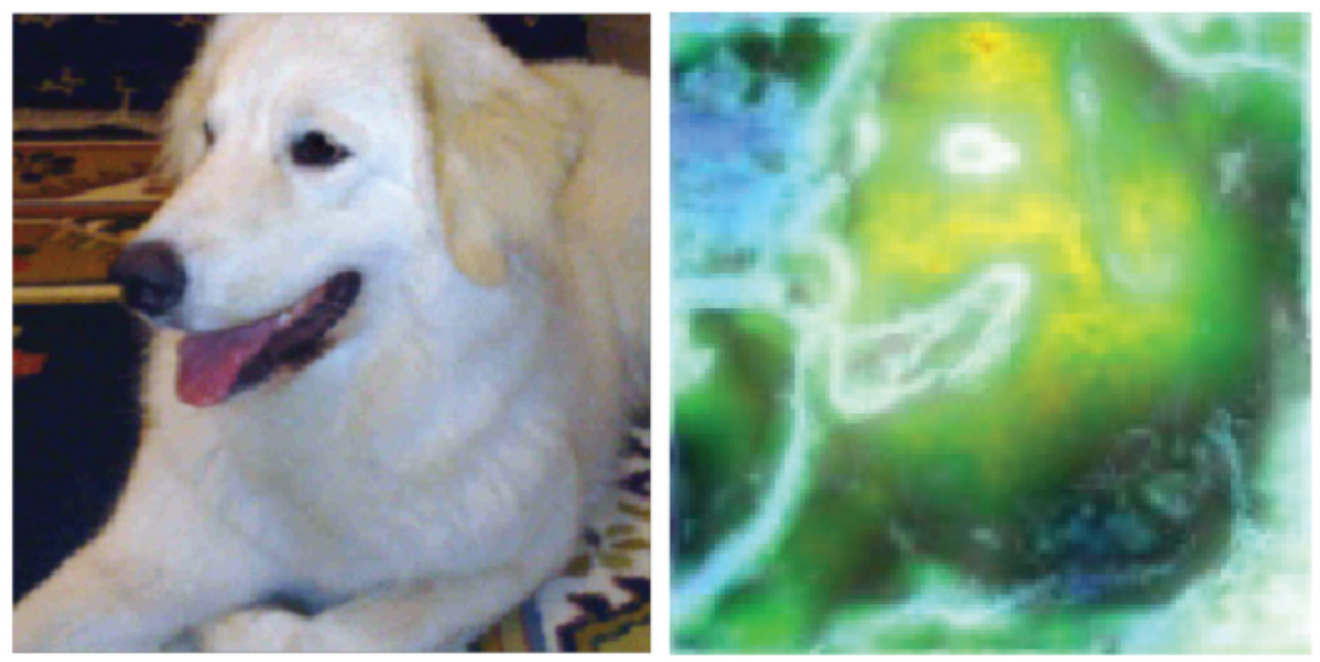
\includegraphics[width = 0.8 \textwidth]{figure/saliencymap}
% \end{figure}
% \end{frame}
%
% \begin{frame}{What is Interpretability?}
% \begin{itemize}
% %\itemsep1em
% \item There is no scientific consensus on the definition of interpretability.
% \item We need to differentiate between interpretations of a model or reality. The latter is distorted by all modeling fallacies involved in predictive modeling, e.g., data quality, under- and overfitting, or model extrapolations.
% \item We use a practical definition of interpretability.
% Think back to the foundations of statistical modeling:  the linear regression model (LM). The LM, with its known equation of beta coefficients, represents a paradigm for statistical interpretability.
% \item It follows that it would be beneficial to create techniques that give us an interpretation similar to the one of an LM.
%
% \end{itemize}
% \end{frame}


% \begin{frame}{Correlation and Dependence}
% \begin{itemize}
% \item \textbf{Correlation:} Often linear correlation (Pearson $\rho$) between pairs of features is meant
% \item \textbf{Dependence:} More general dependence structure (e.g., non-linear relationships)
% \item $X_j$, $X_k$ independent $\Leftrightarrow$ joint probability density function (PDF) is product of marginal PDFs:
% %$$\text{PDF}_{X_j, X_k}(x_j, x_k) = \text{PDF}_{X_j}(x_j) \cdot \text{PDF}_{X_k}(x_k)$$
% $$\P(X_j, X_k) = \P(X_j) \cdot \P(X_k)$$


% $\P(X_j|X_k) = \P(X_j)$ knowing $X_k$ does not tell us anything about $X_j$ and vice versa
% \item $X_j$, $X_k$ independent $\Rightarrow$ $X_j$, $X_k$ uncorrelated \textbf{but} $X_j$, $X_k$ uncorrelated $\nRightarrow$ $X_j$, $X_k$  independent
% %\item Auf einer slide eklären, visuell und mathematisch
% \end{itemize}

% \centering

% \only<1>{
% \textbf{Example:} $X_1$, $X_2 \sim N(0,1)$ independent ($\rho = 0$) \hspace{10pt} $X_1$, $X_2 \sim N(0,1)$ dependent ($\rho = 0.8$) \hspace{30pt}

% 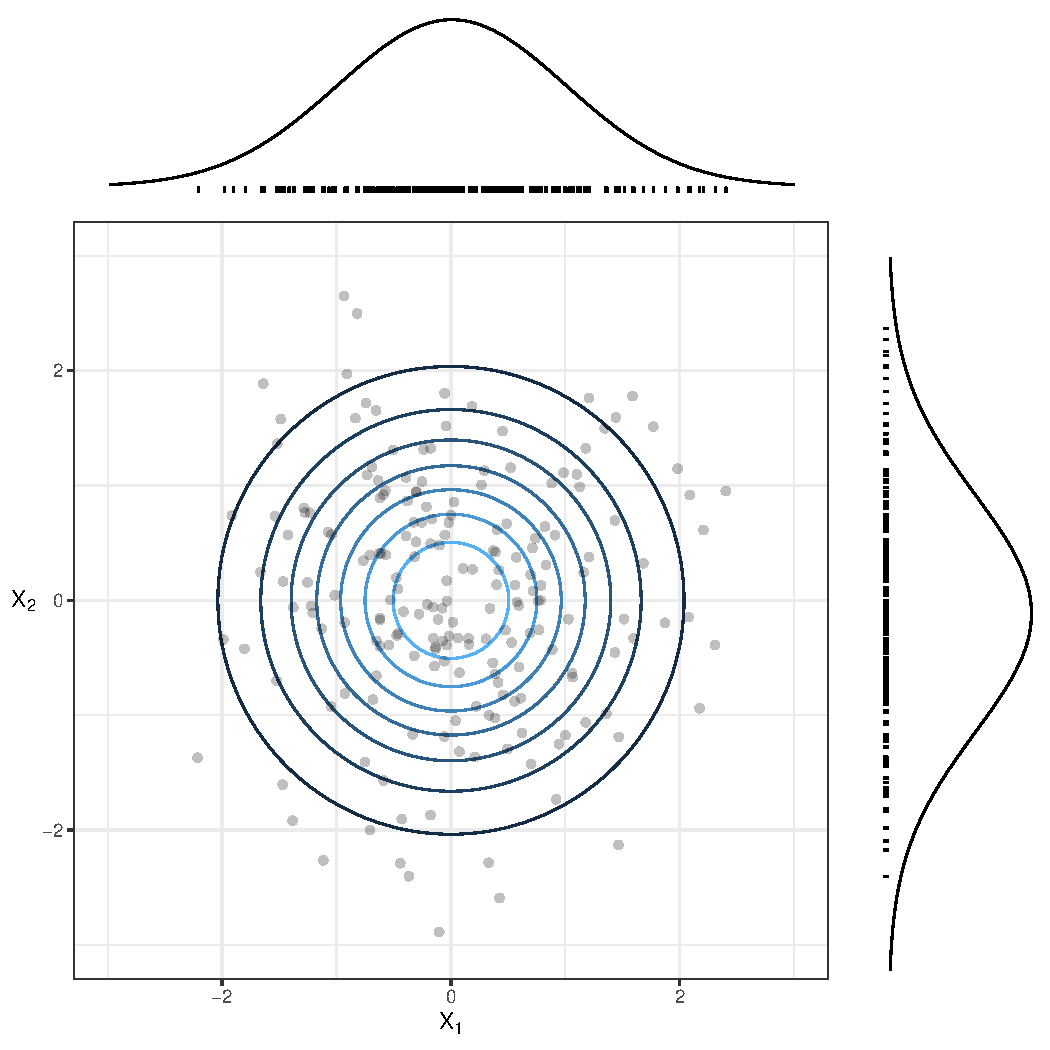
\includegraphics[width = 0.4\textwidth]{figure/independent}
% 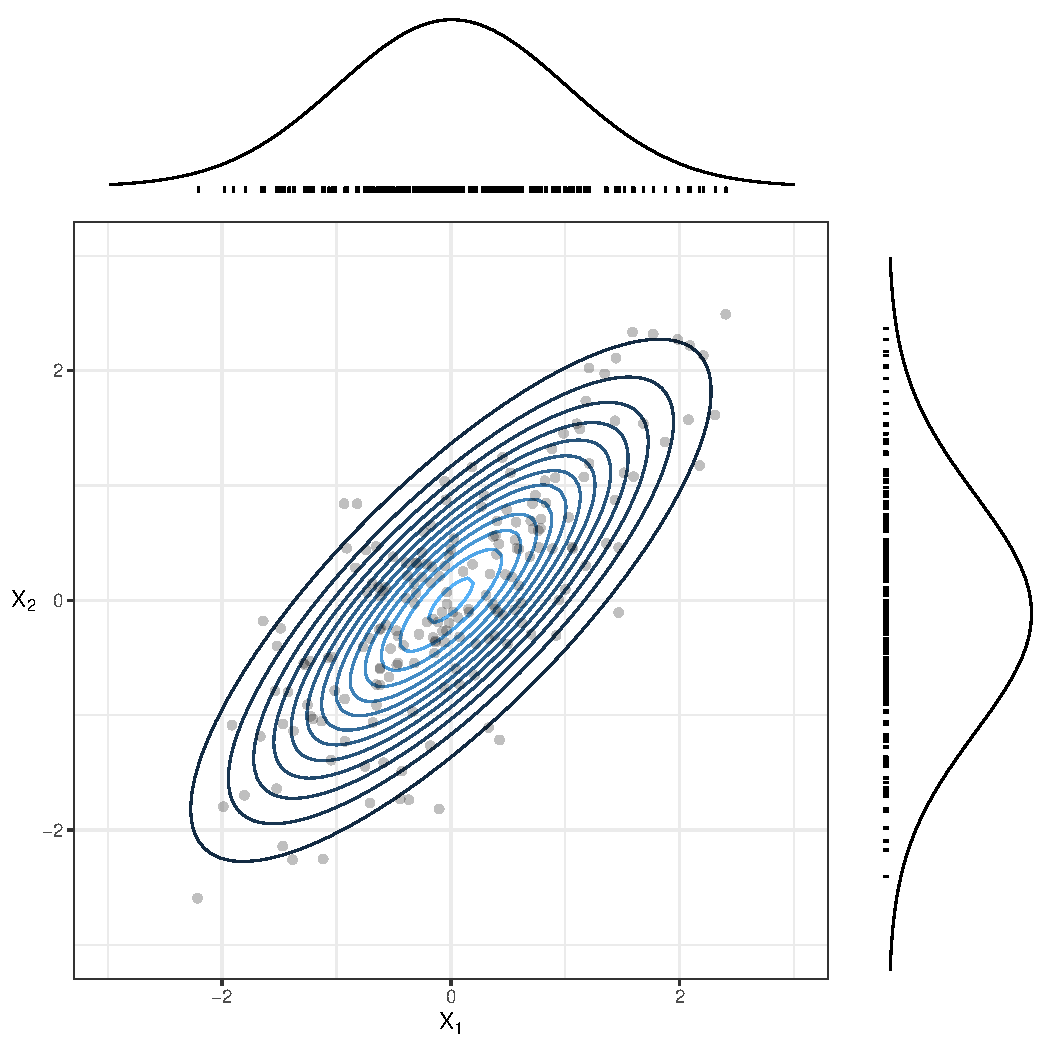
\includegraphics[width = 0.4\textwidth]{figure/dependent}
% }


% \only<2>{
% 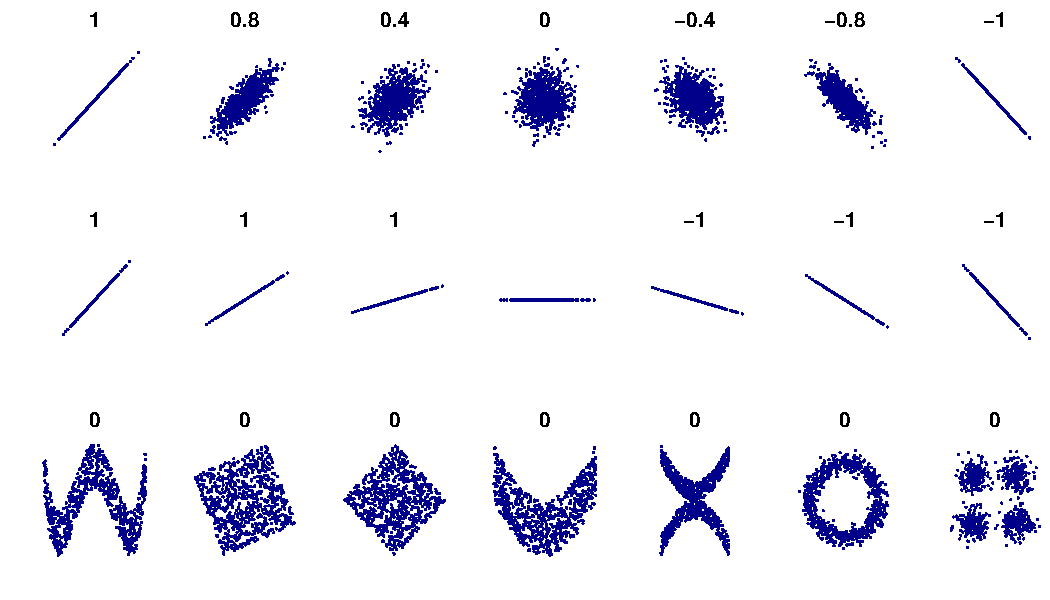
\includegraphics[width = 0.5\textwidth]{figure/dependence_2}
% }
% % correlation reflects the noisiness and direction of a linear relationship (top row), but not the slope of that relationship (middle), nor many aspects of nonlinear relationships (bottom). N.B.: the figure in the center has a slope of 0 but in that case the correlation coefficient is undefined because the variance of Y is zero.
% \end{frame}

\begin{frame}{Joint, Marginal and Conditional Distribution}
    For two discrete random variables $X_1, X_2$:\\
    \medskip
    \begin{columns}[c, totalwidth=\textwidth]
    \begin{column}{0.5\textwidth}
    \textit{Joint distribution}
        \begin{align*}
            p_{X_1, X_2}(x_1,x_2) = \mathbb{P}(X_1 = x_1, X_2 = x_2) %
        \end{align*}
    \textit{Marginal distribution}
        \begin{align*}
            p_{X_1}(x_1) = \mathbb{P}(X_1 = x_1) = \sum_{x_2\in \mathcal{X}_2} p(x_1,x_2)
        \end{align*}
    \textit{Conditional distribution}
        \begin{align*}
            p_{X_1|X_2}(x_1 | x_2) = \mathbb{P}(X_1=x_1| X_2 = x_2) = \frac{p_{X_1, X_2}(x_1,x_2)}{p_{X_2}(x_2)}
        \end{align*}
    $\leadsto$ Analogue in the continuous case with integrals.
    \end{column}
    \begin{column}{0.5\textwidth}
    \begin{table}
    \scriptsize
        \begin{tabular}{|c|c|c|c|}
            \hline 
            $p_{X_1, X_2}$ & $\mathbb{P}(X_2 = 0)$ & $\mathbb{P}(X_2 = 1)$ & $p_{X_1}$ \\
            \hline
            $\mathbb{P}(X_1 = 0)$ & \cellcolor{gray}0.2 & \cellcolor{gray}0.3 & 0.5  \\
            \hline
            $\mathbb{P}(X_1 = 1)$ & \cellcolor{gray}0.1 & \cellcolor{gray}0.4 & 0.5  \\
            \hline
            $p_{X_2}$ & 0.3 & 0.7 & 1  \\
            \hline
        \end{tabular} \\
        \bigskip
        \begin{tabular}{|c|c|c|c|}
            \hline 
            $p_{X_1, X_2}$ & $\mathbb{P}(X_2 = 0)$ & $\mathbb{P}(X_2 = 1)$ & $p_{X_1}$ \\
            \hline
            $\mathbb{P}(X_1 = 0)$ & 0.2 & 0.3 & \cellcolor{gray}0.5  \\
            \hline
            $\mathbb{P}(X_1 = 1)$ & 0.1 & 0.4 & \cellcolor{gray}0.5  \\
            \hline
            $p_{X_2}$ & 0.3 & 0.7 & 1  \\
            \hline
        \end{tabular}\\
        \bigskip
        \begin{tabular}{|c|c|c|c|}
            \hline 
             & $x_2 = 0$ & $x_2 = 1$ \\
            \hline
            $\mathbb{P}(X_1 = 0|X_2 =x_2)$ & \cellcolor{gray} 0.67 & \cellcolor{gray}0.43   \\
            \hline
            $\mathbb{P}(X_1 = 1|X_2 =x_2)$ & \cellcolor{gray} 0.33 & \cellcolor{gray}0.57   \\
            \hline
            $\sum$ & 1 & 1  \\
            \hline
        \end{tabular}
    \end{table}
    \end{column}
    \end{columns} 
    %\bigskip
    
\end{frame}



\begin{frame}{Pearson's correlation coefficient $\rho$}

By \textbf{correlation} often Pearson's correlation is meant (measures only \textbf{linear relationship}) %between pairs of features


%\dfrac{s_{X_1 X_2}}{s_{X_1} \cdot s_{X_2}} \text{ with }

% \begin{itemize}
%     \item Sample covariance of $X_1$ and $X_2$:
%     $s_{X_1 X_2} = \frac{1}{n-1}\sum_{i=1}^{n}{(x_1^{(i)}-\bar{x}_1) \cdot (x_2^{(i)}-\bar{x}_2)}$
%     \item Sample standard deviation $s_{X_1}$ and $s_{X_2}$ of $X_1$ and $X_2$
% \end{itemize}

\begin{columns}[c, totalwidth=\textwidth]
\begin{column}{0.5\linewidth}
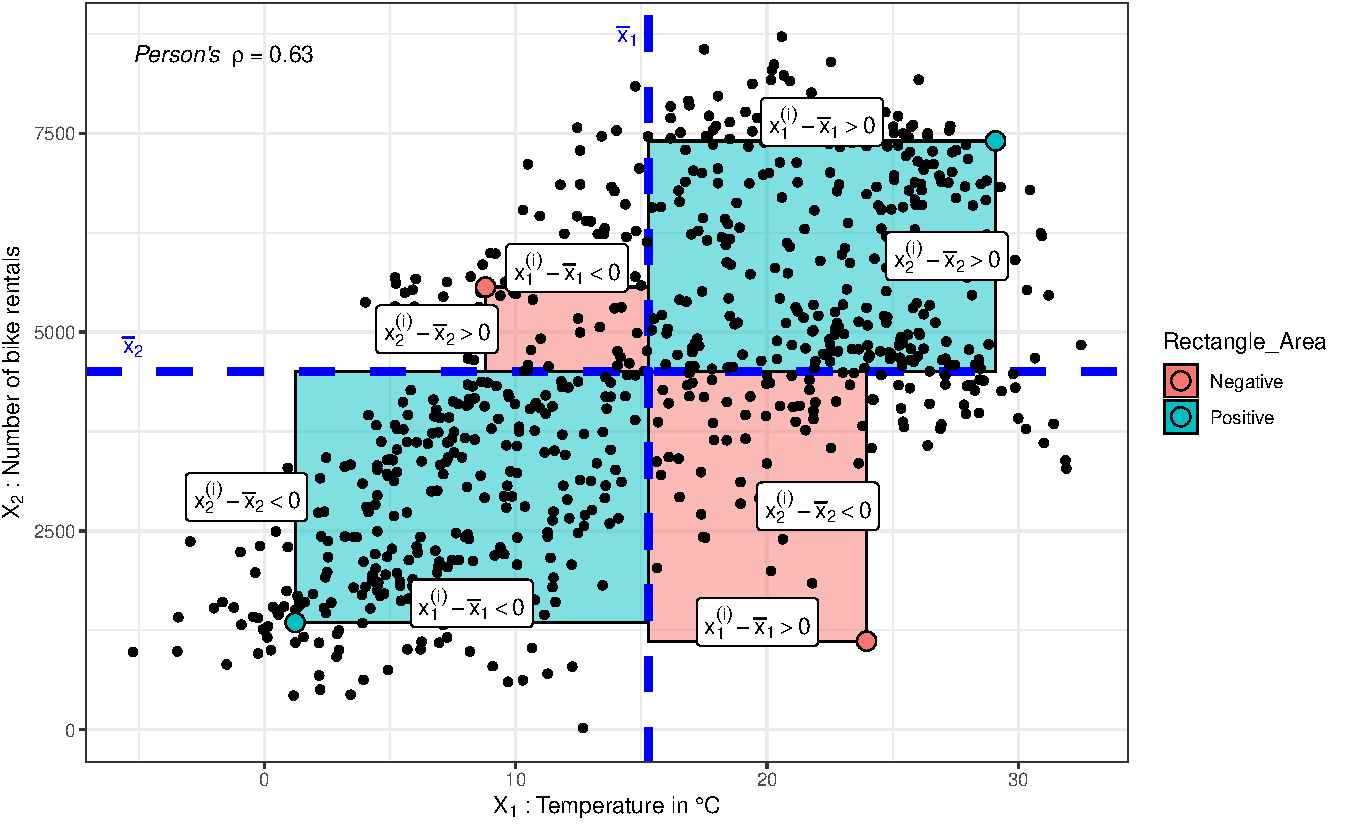
\includegraphics[width = \textwidth]{figure/pearson_cor}
\end{column}
\begin{column}{0.5\linewidth}

\centerline{$\rho(X_1, X_2) = \tfrac{\sum_{i=1}^{n}{(x_1^{(i)}-\bar{x}_1) \cdot (x_2^{(i)}-\bar{x}_2)}}{\sqrt{\sum_{i=1}^{n}{(x_1^{(i)}-\bar{x}_1)^2 \sum_{i=1}^{n}{(x_2^{(i)}-\bar{x}_2)^2 }}}} \in [-1, 1]$}

\medskip

Geometric interpretation of $\rho$:
\begin{itemize}
    \item Numerator is sum of rectangle's area with width $x_1^{(i)}-\bar{x}_1$ and height $x_2^{(i)}-\bar{x}_2$
    \item Areas enter numerator with positive (\textbf{+}) or negative (\textbf{-}) sign, depending on point position
    \item Denominator scales the sum to $ [-1, 1]$
    %\item $\rho = 0$ if area of all rectangles cancels out\\
    %$\leadsto$ $X_1, X_2$ uncorrelated
\end{itemize}
\end{column}
\end{columns}

\medskip
\pause
\begin{itemize}
    \item $\rho = 0$ if area of rectangles of all points cancels out
    $\leadsto$ $X_1, X_2$ linearly uncorrelated
    \item $\rho > 0$ if {\color{ggblue}positive areas} dominate {\color{ggred}negative areas} 
    $\leadsto$ $X_1, X_2$ positive correlated
    \item $\rho < 0$ if {\color{ggred}negative areas} dominate {\color{ggblue}positive areas} 
    $\leadsto$ $X_1, X_2$ negative correlated
\end{itemize}
%\textbf{But:} Pearson's $\rho$ does not measure non-linear dependencies, e.g., $\rho = 0$ but dependent:

\end{frame}


\begin{frame}{Coefficient of determination $R^2$}

Another method to evaluate \textbf{linear dependency} between variables is by calculating the $R^2$

\begin{columns}[c, totalwidth=\textwidth]
\begin{column}{0.5\linewidth}
\only<1>{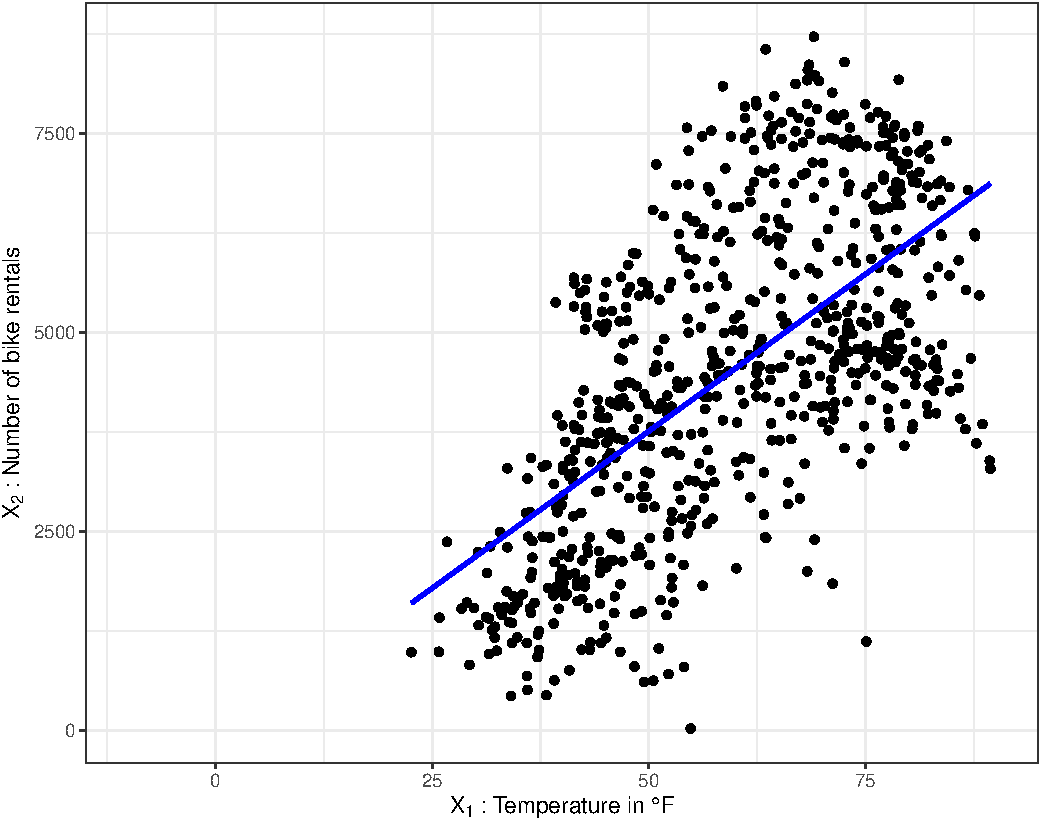
\includegraphics[width = 0.95\textwidth]{figure/r_squared_Fahrenheit}}
\only<2>{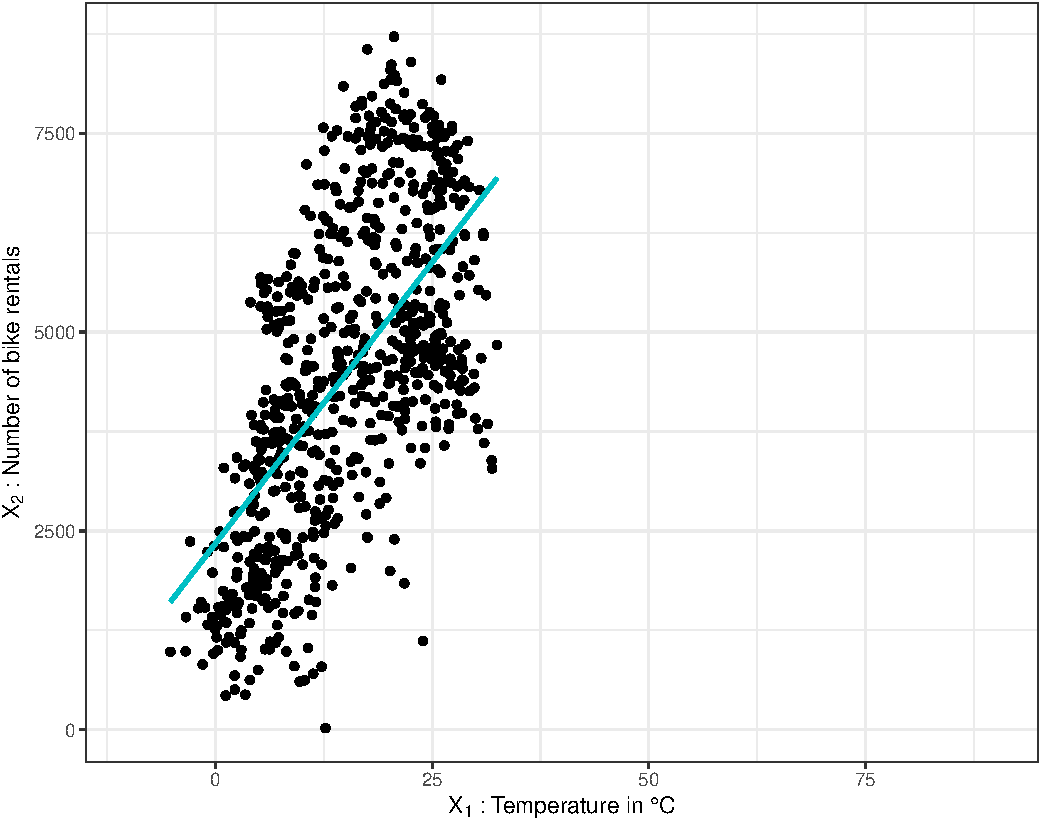
\includegraphics[width = 0.95\textwidth]{figure/r_squared_compare}}
\only<3>{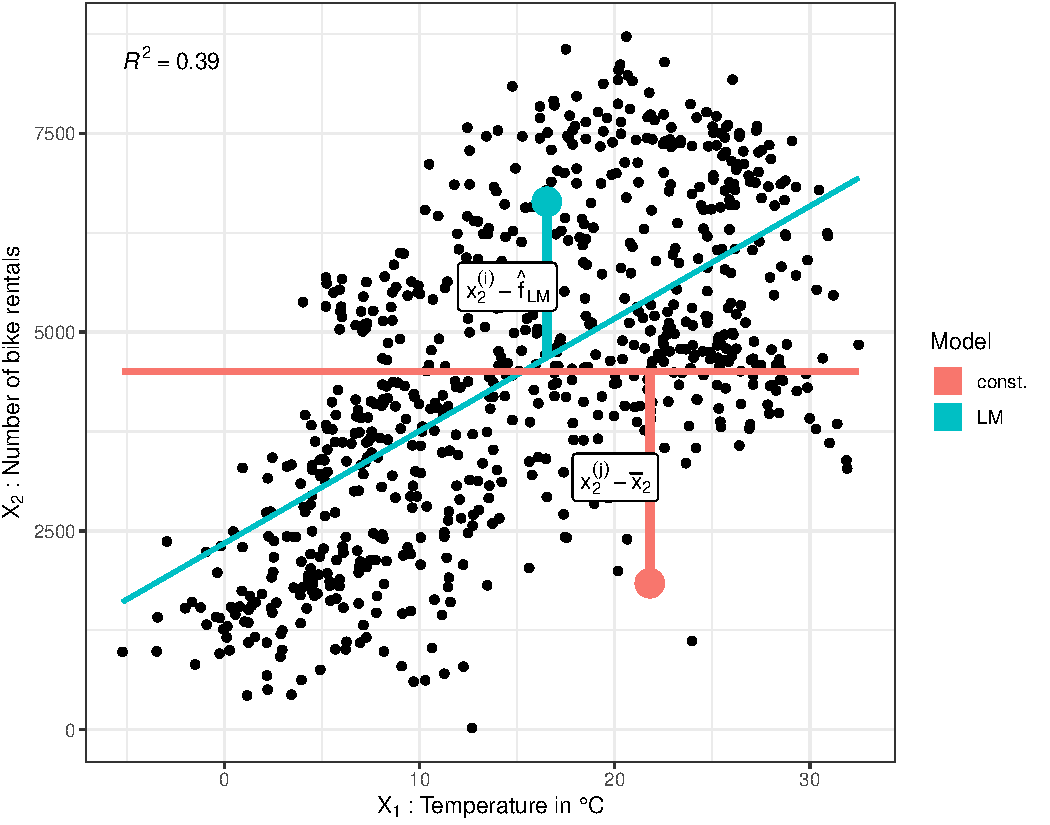
\includegraphics[width = 0.95\textwidth]{figure/r_squared}}
\end{column}
\begin{column}{0.5\linewidth}

\medskip

Idea for two-dimensional case:
\begin{itemize}
    \setlength\itemsep{0.7mm}
    \item Fit a linear model:
    $\hat{x}_2 = \hat{f}_{LM}(x_1) = \theta_0 + \theta_1 x_1$
    %($x_2 \sim x_1$) 
    % $\hat{f}_{LM}(x_1) = 2345 + 141.3 x_1$
    \item[] $\leadsto$ Slope = $0$ $\Rightarrow$ no dependence
    \item[] $\leadsto$ Very large slope $\Rightarrow$ strong dependence
    \item Exact $\theta_1$ score problematic 
    \pause
    \item[] $\leadsto$ Rescaling of $x_1$ or $x_2$ changes $\theta_1$ 
    \only<2>{\item e.g. °F $\rightarrow$ °C $\Rightarrow$ ${\color{blue}\theta_1=78.5}\rightarrow{\color{ggblue}\theta_1^*=141.3}$}
    \pause
    \item Set $SSE_{LM}$ in relation to $SSE$ of a constant model $\hat{f}_c = \bar{x}_2$
    \item[] $SSE_{LM} = \sum_{i=1}^n ({\color{ggblue}x_2^{(i)} - \hat{f}_{LM}(x_1^{(i)})})^2$
    \item[] $SSE_{c} = \sum_{i=1}^n ({\color{ggred}x_2^{(i)} - \bar{x}_2})^2$
\end{itemize}

\end{column}
\end{columns}

\begin{align*}
    &\Rightarrow \text{ Measure of fitting quality of LM: } R^2 = 1-\frac{SSE_{LM}}{SSE_{c}} \in [-1, 1] \\
    &\Rightarrow \rho(X_1, X_2) = R
\end{align*}

\end{frame}


\begin{frame}{Mutual Information}
    \begin{itemize}
        \item MI describes amount of information about one random variable obtained through another one or how different the joint distribution is from pure independence
        \item $MI(X_1 ; X_2 )$ is the Kullback-Leibler distance between joint distribution and product distribution $p_{X_1} p_{X_2}$:
        \begin{align*}
            MI(X_1 ; X_2 ) &= \sum_{x_1 \in \mathcal{X}_1} \sum_{x_2 \in \mathcal{X}_2} p(x_1, x_2) log\left(\frac{p(x_1, x_2)}{p(x_1) p(x_2)} \right) \\
            &= D_{KL} \left( p(x_1, x_2) \, || \, p(x_1) p(x_2) \right) \\
            &= \mathbb{E}_{p(x_1, x_2)} \left[ log\left(\frac{p(x_1, x_2)}{p(x_1) p(x_2)} \right) \right]
        \end{align*}
        \item MI measures amount of "dependence" between variables. It is zero if and only if the variables are independent.
        \item Unlike (Pearson) correlation, MI is not limited to real-valued random variables.
    \end{itemize}
\end{frame}



\begin{frame}{Correlation and Dependence}

Scatterplot with multivariate distribution (contour lines) and marginal density $X_1$, $X_2 \sim N(0,1)$ 

\only<1>{\begin{center}
\begin{minipage}[t]{0.3\textwidth}
\centering
 $\rho(X_1, X_2) = 0$
\end{minipage}
\begin{minipage}[t]{0.3\textwidth}
\centering
 $\rho(X_1, X_2) = 0.8$
\end{minipage}
\begin{minipage}[t]{0.3\textwidth}
\centering
 $\rho(X_1, X_2) = -0.8$
\end{minipage}
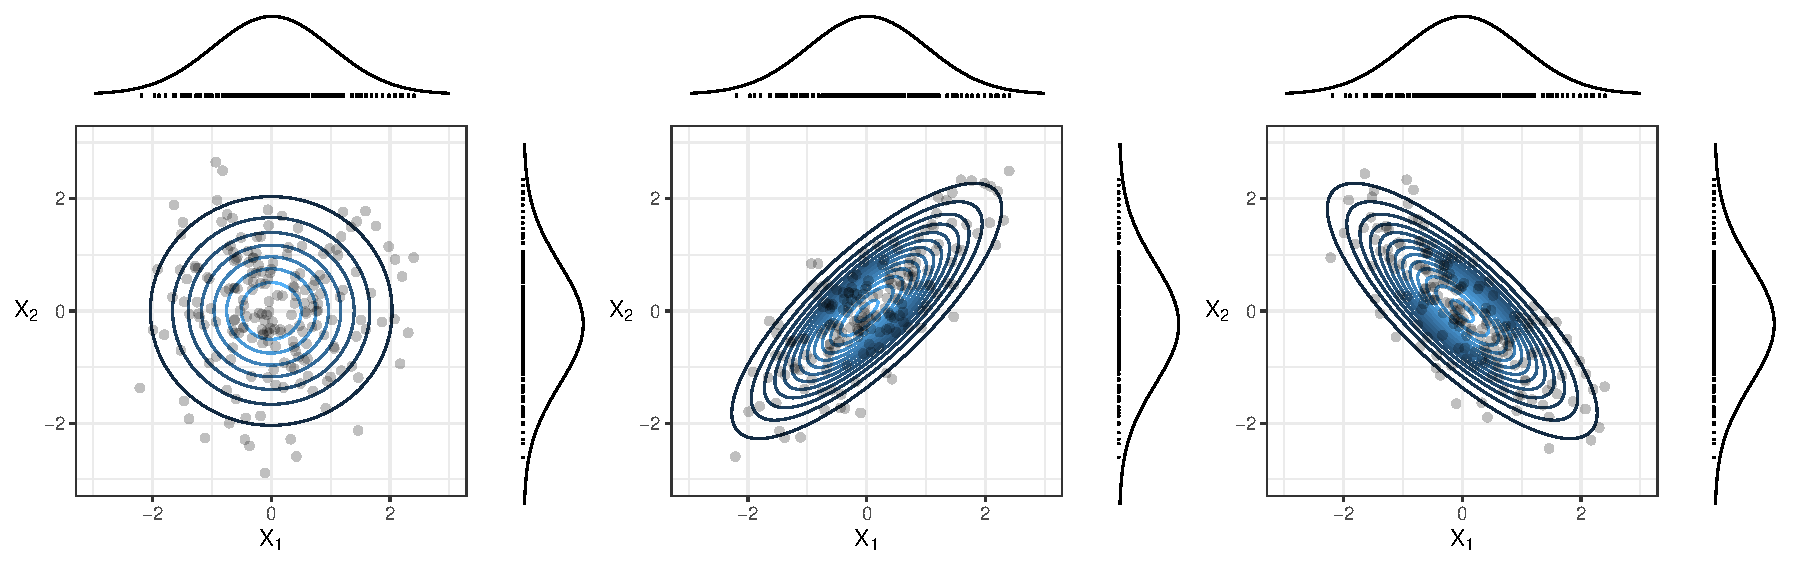
\includegraphics[width = 0.9\textwidth]{figure/dnorm_correlation.pdf}
\end{center}}

\only<2>{\begin{center}
\begin{minipage}[t]{0.15\textwidth}
\centering{\scriptsize
 $\rho(X_1, X_2) = 0$}
\end{minipage}
\begin{minipage}[t]{0.15\textwidth}
\centering{\scriptsize
 $\rho(X_1, X_2) = 0.8$}
\end{minipage}
\begin{minipage}[t]{0.15\textwidth}
\centering{\scriptsize
 $\rho(X_1, X_2) = -0.8$}
\end{minipage}\\
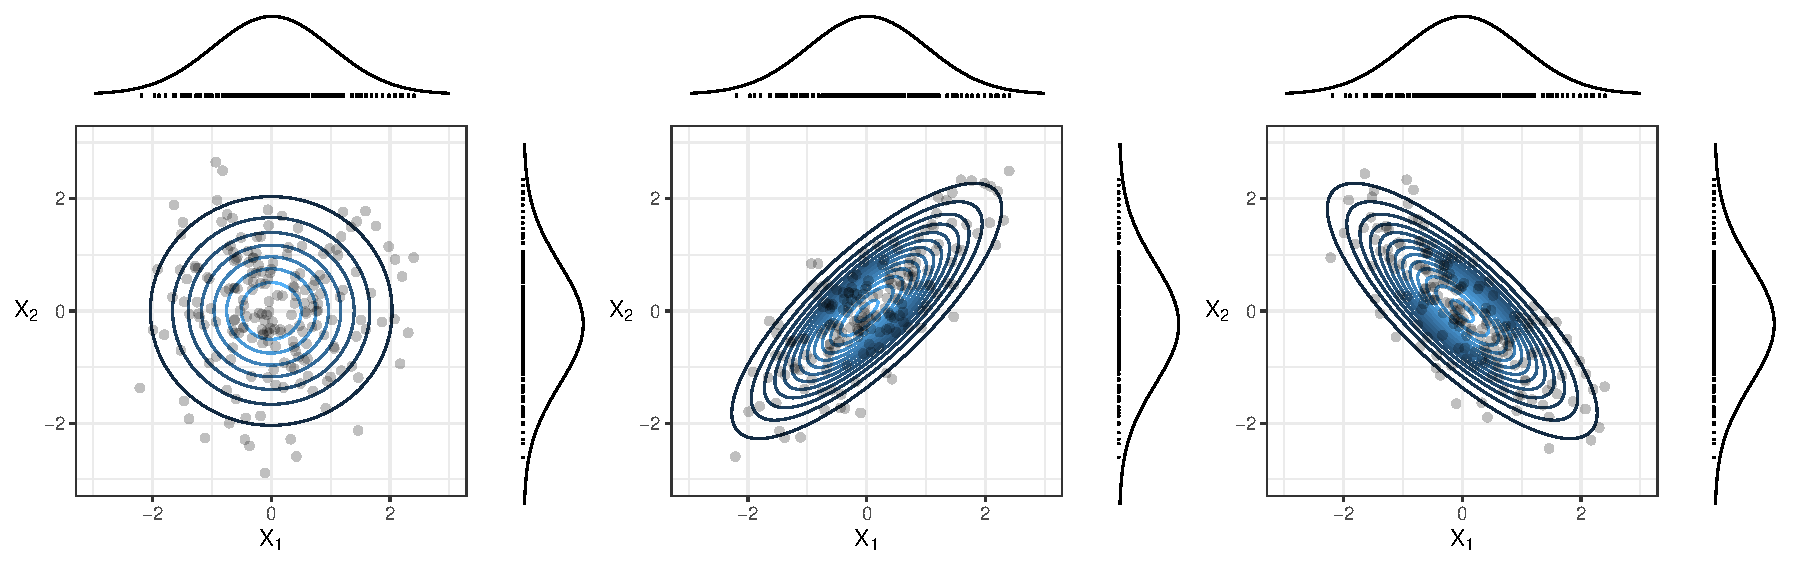
\includegraphics[width = 0.45\textwidth]{figure/dnorm_correlation.pdf}
\end{center}


Examples with Pearson's correlation $\rho = 0$ but non-linear dependencies (MI $\neq 0$):\\
\medskip
\centering
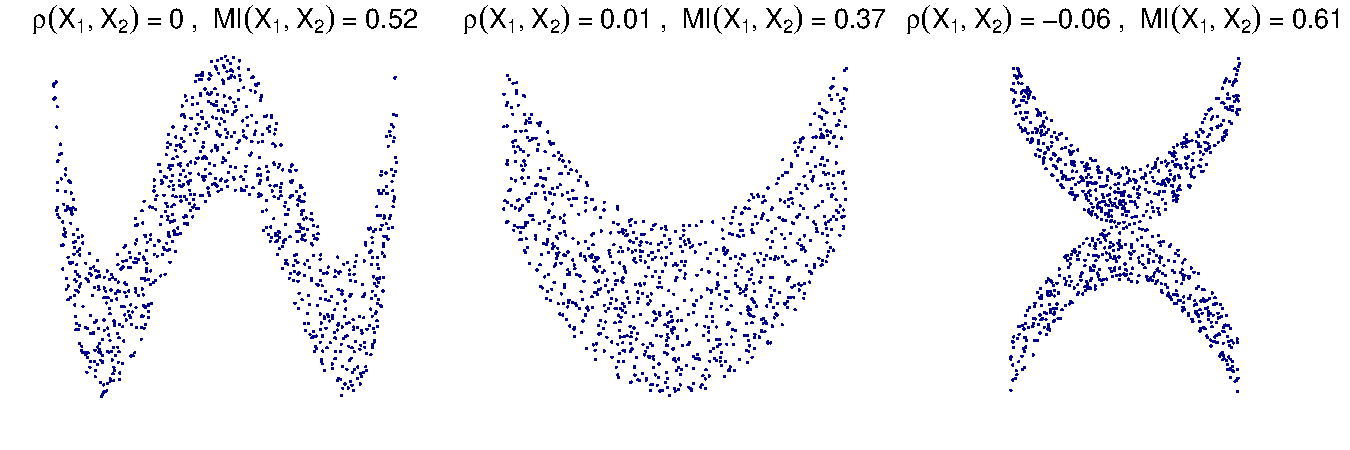
\includegraphics[width = 0.8\textwidth]{figure/dependence_3}}
\end{frame}


\begin{frame}{Correlation and Dependence}
\textbf{Dependence:} Describes general dependence structure of features (e.g., non-linear relationships)

%\textbf{Definition:}
\begin{itemize}[<+->]
\item Definition: $X_j$, $X_k$ independent $\Leftrightarrow$ joint distribution is product of marginals:\\ \vspace{5pt}
\centerline{$\P(X_j, X_k) = \P(X_j) \cdot \P(X_k)$}
\vspace{5pt}
\item Equivalent definition (knowing $X_k$ does not tell us anything about $X_j$ and vice versa): \\
\vspace{5pt}
\phantom{AAA} $\P(X_j|X_k) = \P(X_j) \text{ and } \P(X_k|X_j) = \P(X_k)$ \hfill (follows from conditional probability) \phantom{AAA}
\vspace{5pt}
%$$\P(X_j|X_k) = \P(X_j) \hfill \text{(knowing $X_k$ does not tell us anything about $X_j$ and vice versa)}$$
%\medskip
\item Measuring complex dependencies is difficult but different measures exist, e.g., \\
$\leadsto$ Spearman correlation (measures monotonic dependencies via ranks) \\
$\leadsto$ Information-theoretical measures like mutual information \\
$\leadsto$ Kernel-based measures like Hilbert-Schmidt Independence Criterion (HSIC)
% nice further reading https://jejjohnson.github.io/research_journal/appendix/similarity/hsic/
\item \textbf{N.B.:} $X_j$, $X_k$ independent $\Rightarrow$ $\rho(X_j, X_k) = 0$ \textbf{but} $\rho(X_j, X_k) = 0$ $\nRightarrow$ $X_j$, $X_k$  independent \\
But equivalency holds if distribution is jointly normal
\item  $MI(X_j, X_k) = 0$ if and only if $X_j$, $X_k$ independent
\end{itemize}
\end{frame}


\begin{frame}{Correlation and Dependence}
	
\textbf{Example:}
\begin{columns}[T, totalwidth=\linewidth]
\begin{column}{0.49\linewidth}
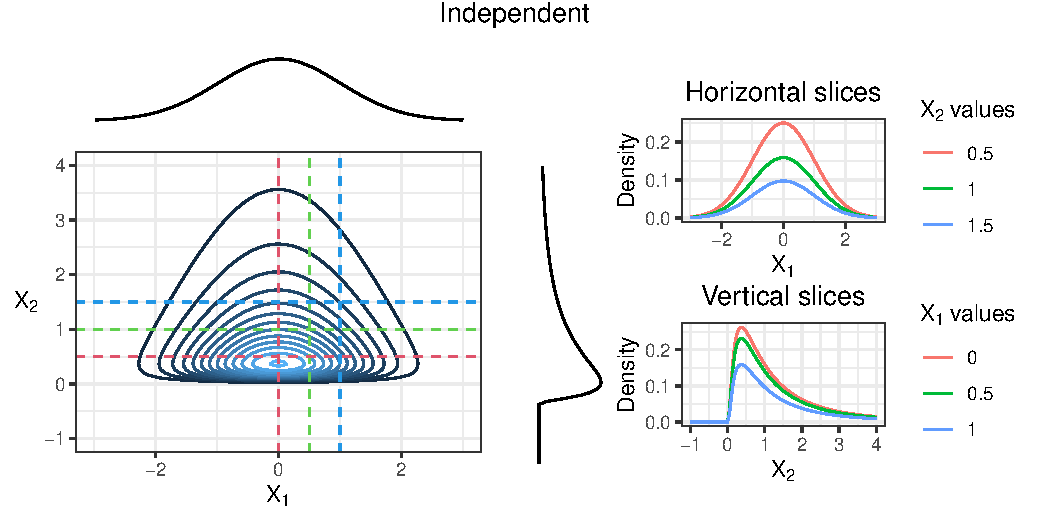
\includegraphics[width=\linewidth]{figure/independent_slice.pdf}
Conditional distributions at different vertical and horizontal slices (after normalizing area to 1) match their marginal distributions
\medskip

$\Rightarrow$ $\P(X_1|X_2) = \P(X_1) \text{ and } \P(X_2|X_1) = \P(X_2)$
\end{column}
\hfill\pause
\begin{column}{0.49\linewidth}
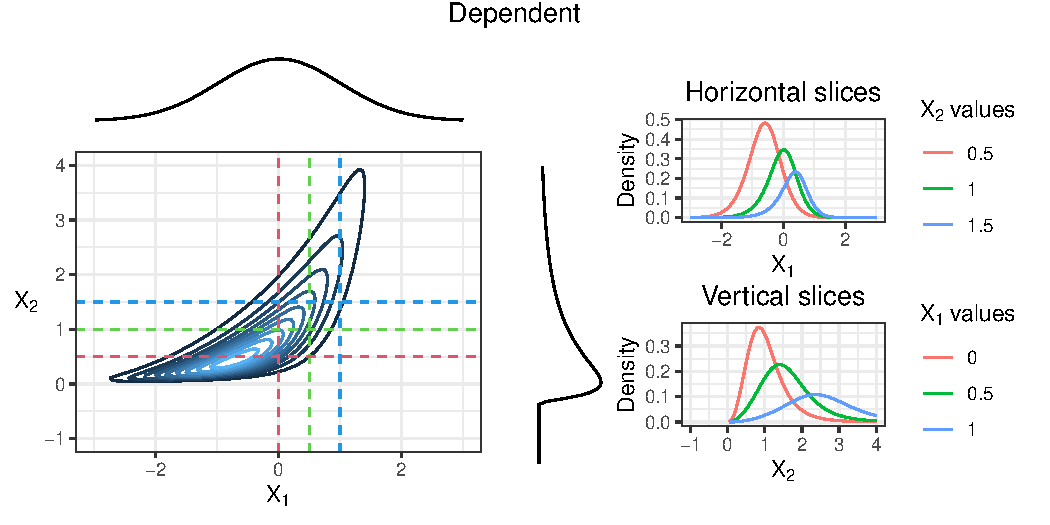
\includegraphics[width=\linewidth]{figure/dependent_slice.pdf}
Conditional distributions do not match their marginal distributions
\end{column}
\end{columns}


\end{frame}



\begin{frame}{Interpretations with Dependent Features}
\begin{itemize}

% \item Be clear about interpretation goal: Explain model or underlying relationship in data?
% %We need to differentiate between interpretations of a model or reality
% \\
% $\leadsto$ Latter might be distorted by modeling fallacies, 
% e.g., 
% %due to bad data quality, 
% under- and overfitting or extrapolation

%\pause
\item Highly correlated features contain similar information \\
$\leadsto$ Model might pick only one feature (regularization) (even if it is causally irrelevant)
%Some models might use only one correlated feature (even if it is causally not relevant)
\\
%Can confuse a model so that only one correlated feature is used (even if it is not relevant) \\
$\leadsto$ Produced explanations can be misleading (true to the model, but not to the data) % generating process
\\
$\leadsto$ Different IML models often produce different results in these situation, and not always trivial to understand which / why 
%Even for two causally and equally relevant correlated features it is not guaranteed that their explanations will be similar
% \pause
% \item Assume two causally and equally relevant but highly correlated features \\
% $\leadsto$ One might expect that their explanations (e.g., feature importance) will be similar \\
% %One might expect that explanations of two correlated features (e.g., feature importance) are similar as they share similar information \\
% $\leadsto$ Generally not true as the model can learn different relationships


% \begin{tikzpicture}[remember picture,overlay,shift=(current page.center)] %opacity=.2,text opacity=1
% \node[fill=white, opacity=1,text opacity=1] at (current page.center) {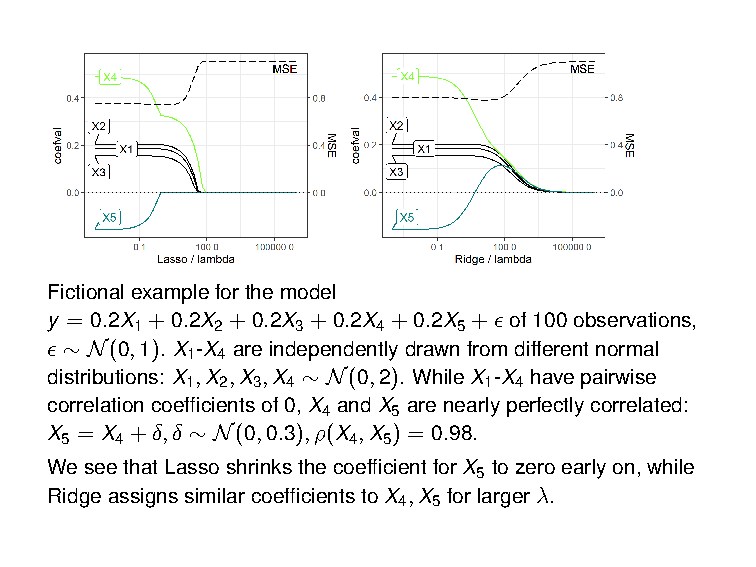
\includegraphics[width=0.6\textwidth]{figure/ridge_lasso}};
% \end{tikzpicture}
\pause

% \only<3>{
%  \begin{BlueBox}{Example}
%   \begin{columns}[c, totalwidth=\textwidth]
% \begin{column}{0.5\textwidth}
% 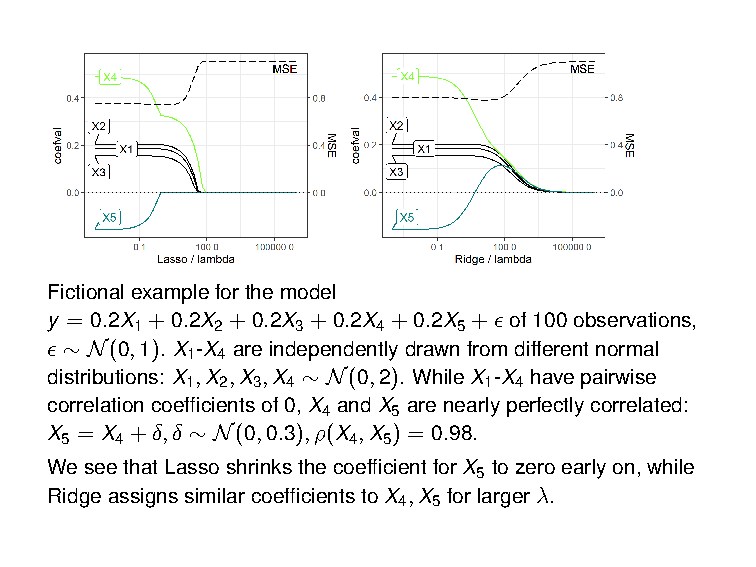
\includegraphics[trim=0px 110px 30px 0px, clip, width=\textwidth]{figure/ridge_lasso}
% \end{column}
% \begin{column}{0.5\textwidth}
% 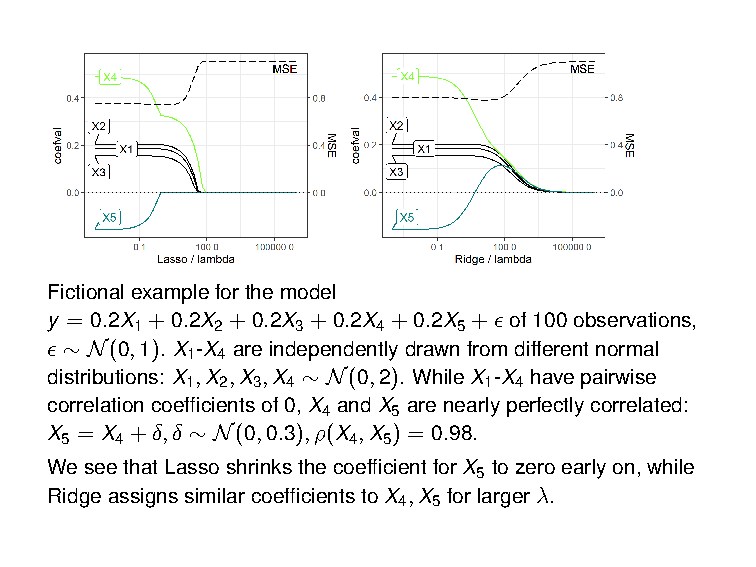
\includegraphics[trim=0px 0px 0px 115px, clip, width=\textwidth]{figure/ridge_lasso}
% \end{column}
% \end{columns}}
% \end{BlueBox}
% }

%\only<3>{
\colorbox{blue!20}{\begin{columns}[c, totalwidth=\linewidth]
\begin{column}{0.5\linewidth}
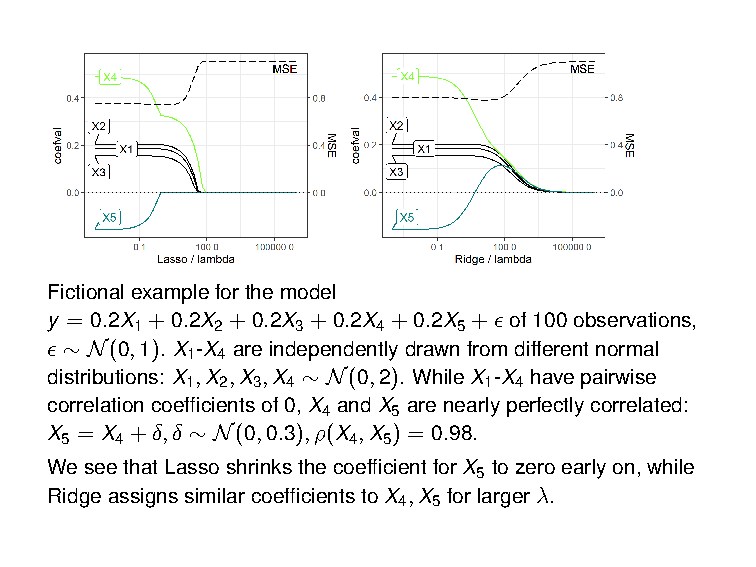
\includegraphics[trim=0px 110px 30px 0px, clip, width=\linewidth]{figure/ridge_lasso}
\end{column}
\begin{column}{0.5\linewidth}
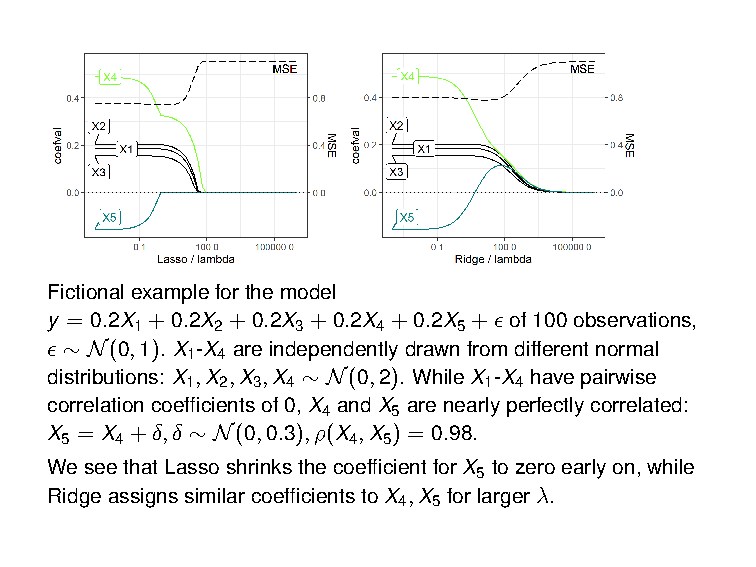
\includegraphics[trim=0px 0px 0px 115px, clip, width=\linewidth]{figure/ridge_lasso}
\end{column}
\end{columns}}
%}

\end{itemize}
\end{frame}



\begin{frame}{Extrapolation due to Dependencies}
%\begin{center}
\centerline{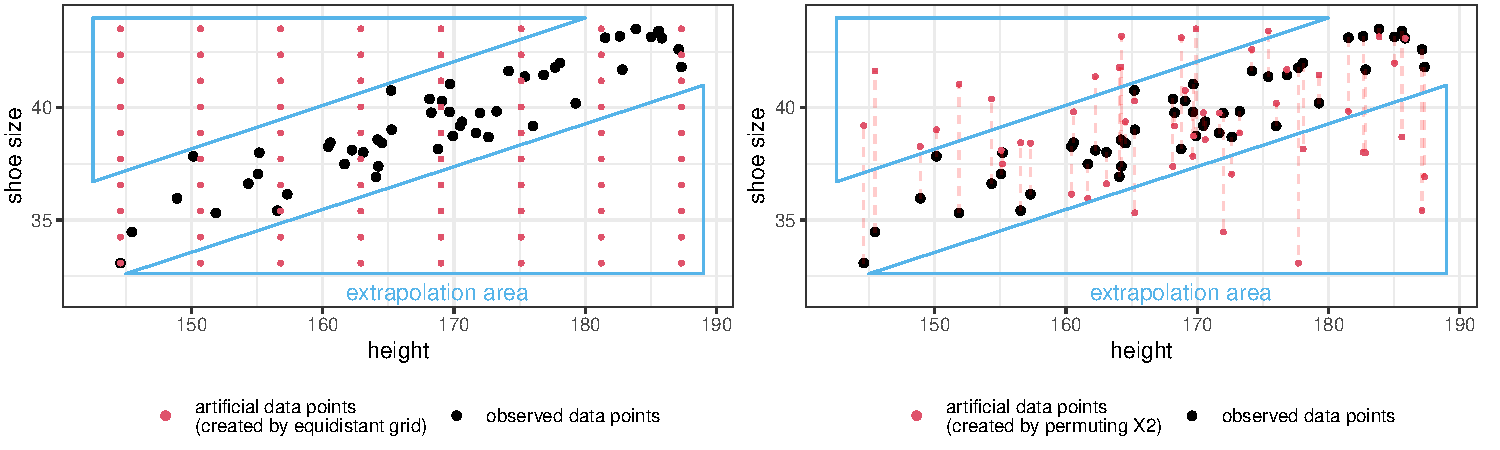
\includegraphics[width=0.8\textwidth]{figure/extrapolation}}
%\end{center}

\begin{itemize}
%\itemsep1em
\item Many interpretation methods are based on
%rely on varying feature values and create
artificially created data points \\
$\leadsto$ Many of these points can lie in low-density regions if features are dependent\\
$\leadsto$ Model predictions in such regions are subject to a high uncertainty\\ % in regions with no or few training data
$\leadsto$ Explanations may be biased as they often rely on predictions where model extrapolated\\
\pause
%\item 
%\item Essentially, we are interested in the prediction uncertainty\\
%, i.e., the less the training data on a feature subspace, the higher the prediction uncertainty.
%$\leadsto$ Models are rarely able to quantify uncertainty of predictions %Models are rarely capable of quantifying prediction uncertainty
\item There is no definition of when a model extrapolates and to what degree \\
$\leadsto$ Severity of extrapolation depends on model, some extrapolate more than others \\
$\leadsto$ Training density might serve as proxy to identify regions where extrapolation is likely \\
\phantom{$\leadsto$} But: Density estimation in many dimensions is often infeasible
%$\leadsto$ Some models might extrapolate more than others
%\item Density of training data might serve as proxy to identify regions where extrapolation is likely\\
%$\leadsto$ Density estimation in many dimensions is often infeasible
\end{itemize}

\end{frame}
% \begin{frame}{Extrapolation}
% \begin{itemize}
% %\itemsep1em
% \item Predictions of an ML model in regions with a low density of training points are subject to a high variance.
% \item Essentially we are interested in the prediction uncertainty, i.e., the less the training data on a feature subspace, the higher the prediction uncertainty. Unfortunately, virtually no ML models are capable of quantifying prediction uncertainty.
% \item There is no consensus definition of when a model extrapolates and to what degree. Furthermore, the severity of the problem depends on the model itself. Some models might extrapolate more reliably than others.
% \item Theoretically, we could use the training density as a proxy. However, density estimation in many dimensions is often infeasible.
% \end{itemize}

% \end{frame}

%%% dann das gleiche für interactions

%% wir können auch ein bsp mit feature importannce machen, wo korrelation alles schwieriger macht. im guyon paper und im i2ml featsel teil ist es drin

%% was kann mindestens zu korrel sagen:
%
% a) das extrapol problem. haben wir folien zu
% b) bei korrel kann man sagen: die vars haben die gkleich info, also breaucht man nur eine. das ist eine explanation. die kann aber falsch sein. siehe guyon bsp
% c) bei korrel könnte man sagen: die erklärungen zu vars sind die gleichen. zb deren importance. das ist aber auch nicht gegeben
% ---> generell: vorsicht!

%--------------------------------

% bei interactions:
% 1) definition davon bringen
% man kann das operationals / an der modell struktur erklären. als bsp lin modell und tree
% allgemeine definition von fanoava
% sagen dass eine funktin keine IA hat, wenn sie separierbar. verbindung zur optimierung bringen
% sagen dass man aus der fanbova die interactioons ablesen kann und auf die H-statistic für weiteres vereweisen



% \begin{frame}{Correlation vs. Interaction}
% \begin{itemize}
% %\itemsep2em
% \item Correlated (or dependent) features and feature interactions can cause misleading explanations. %One needs to be careful not to confuse them.
% \item Correlated features implies joint is not product of marginals: $\text{PDF}(x_1, \dots, x_p) \neq \text{PDF}(x_1) \cdot \ldots \cdot \text{PDF}(x_p)$.
% \item
% Many interpretation methods rely on varying feature values and may create data points that are out-of-distribution or located in low-density regions if features are correlated.\\
% $\leadsto$ May produce biased explanations that rely on predictions where the model extrapolated.
% % \item An interaction is a product term between features inside the prediction function. As such, interactions are detached from the constitution of the data, i.e., regardloss of the degree of correlation, the effect of a feature on the target will depend on the values of one or multiple other features.
% \end{itemize}
% \end{frame}

% \begin{frame}{Correlation vs. Interaction}

% 1000 randomly sampled observations with positive correlation between $x_1$ and $x_2$:
% \medskip
% \begin{figure}
% 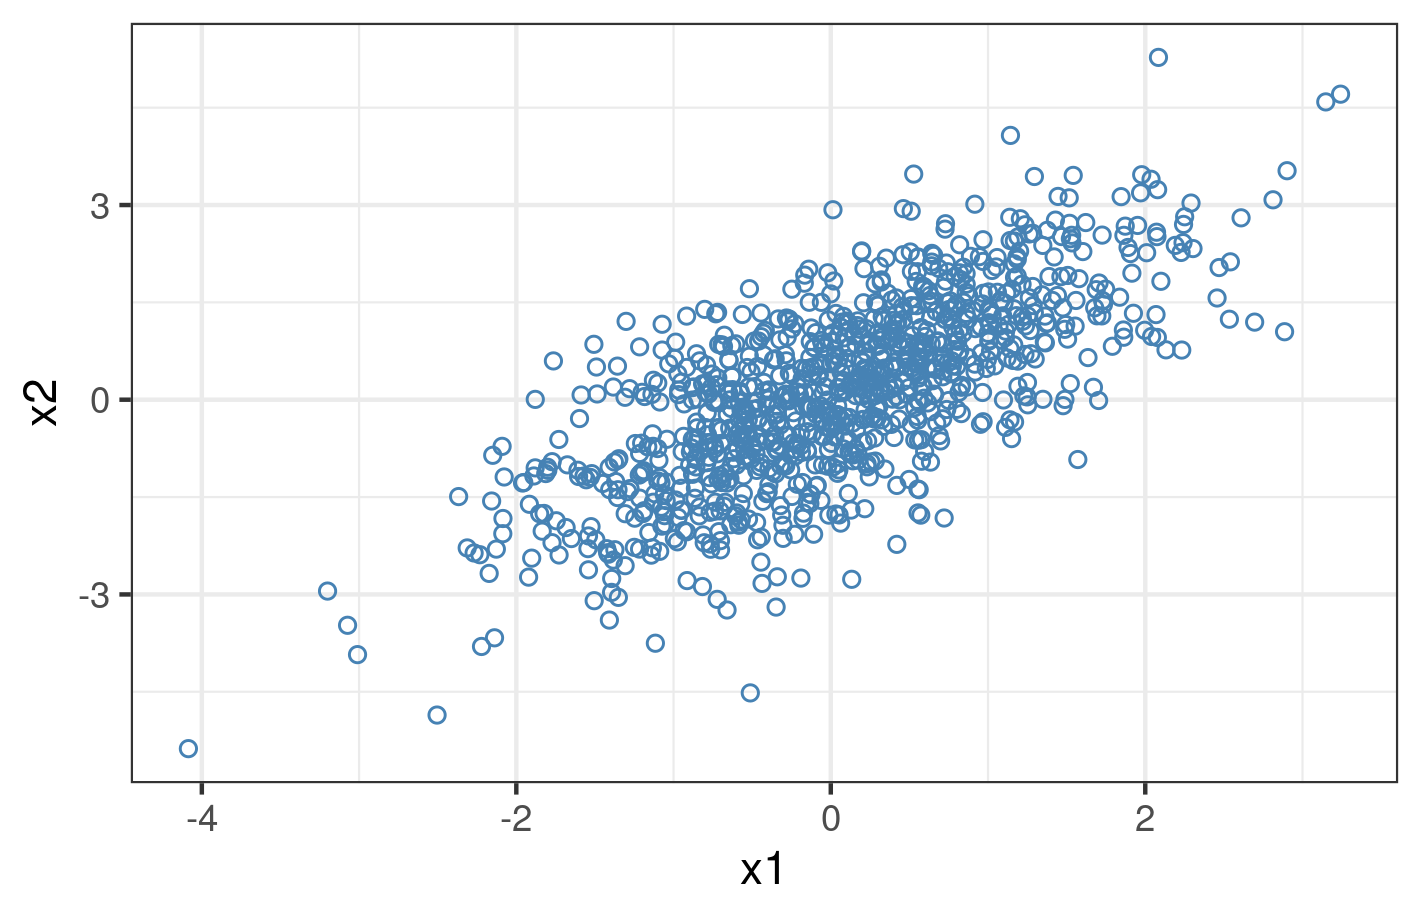
\includegraphics[width = 0.7\textwidth]{figure/correlation}
% \end{figure}
% \end{frame}


\endlecture
\end{document}
